% Editable team document. Normal simulation runs do not overwrite this file.
% Explicit regeneration replaces manual edits. Keep images/ with this project.
\documentclass[a4paper,11pt]{article}
\usepackage[T1]{fontenc}
\usepackage[utf8]{inputenc}
\usepackage{lmodern}
\usepackage[margin=20mm]{geometry}
\usepackage{graphicx,longtable,array,booktabs,ragged2e,seqsplit,listings}
\usepackage{xcolor,hyperref}
\definecolor{navy}{HTML}{19364F}
\hypersetup{colorlinks=true,linkcolor=navy,urlcolor=navy,pdftitle={Smart Grids Team Guide}}
\lstset{basicstyle=\ttfamily\small,breaklines=true,columns=fullflexible,keepspaces=true}
\setlength{\parindent}{0pt}
\setlength{\emergencystretch}{3em}
\setlength{\tabcolsep}{4pt}
\renewcommand{\arraystretch}{1.15}
\begin{document}
\subsection*{SMART GRIDS / MIXED BUILDING COMMUNITY}
\par\medskip

{\LARGE\bfseries Prosumer community simulator\newline{}with heterogeneous buildings\par}\medskip
\par\medskip

{\small 24 October 2026\par}
\par\medskip

The design contains \textbf{150 aggregate building meters: 100 prosumers and 50 consumers}. The original PV-equipped buildings remain unchanged; the added consumers have no PV or batteries. There are 75 small houses, 45 blocks, 15 supermarkets and 15 schools, including \textbf{972 residential dwelling units}. Exactly 55 prosumers own batteries. Each block shares one roof and one meter.
\par\medskip

{\small \textbf{For the team:} sections 11-22 explain every parameter. The demand-response comparison, hourly behavior, worked example and limitations are explained on sections 23-25 when that experiment is present.\par}
\par\medskip

\subsection*{Objective and experiment}
\par\medskip

Encourage neighborhood P2P electricity trading using price guidance and funded seller rewards, then evaluate storage priority and financial outcomes. Self-balancing, P2P, aggregator and grid settlement preserve energy and cash. Every completed internal trade appears in an hourly Proof-of-Work block.
\par\medskip

\begingroup\small
\begin{longtable}{>{\RaggedRight\arraybackslash}p{\dimexpr0.108481\linewidth-2\tabcolsep\relax}>{\RaggedRight\arraybackslash}p{\dimexpr0.197239\linewidth-2\tabcolsep\relax}>{\RaggedRight\arraybackslash}p{\dimexpr0.177515\linewidth-2\tabcolsep\relax}>{\RaggedRight\arraybackslash}p{\dimexpr0.516765\linewidth-2\tabcolsep\relax}}
\toprule
\textbf{Scenario} & \textbf{Storage} & \textbf{Regulation} & \textbf{Charging priority} \\ \midrule
\endfirsthead
\toprule
\textbf{Scenario} & \textbf{Storage} & \textbf{Regulation} & \textbf{Charging priority} \\ \midrule
\endhead
A & 55 owners & Off & Self-consumption first \\ \addlinespace[3pt]
B & 55 owners & On & Self-consumption first \\ \addlinespace[3pt]
C & Disabled & Off & Counterfactual \\ \addlinespace[3pt]
D & Disabled & On & Counterfactual \\ \addlinespace[3pt]
E & 55 owners & Off & P2P before charging \\ \addlinespace[3pt]
F & 55 owners & On & P2P before charging \\ \addlinespace[3pt]
\bottomrule
\end{longtable}
\endgroup

\subsection*{Actual result for the new community}
\par\medskip

With storage, regulation changes P2P energy from \textbf{863.982 to 2,858.451 kWh}, and its share from 13.985\% to 46.269\%. Cost effects differ by scenario and accounting boundary; all values below come from the recorded execution.
\par\medskip

\textbf{Evidence boundary:} geometry, demand profiles, weather and price history are synthetic engineering assumptions. They are not measured building data. This mixed community is a new experiment and cannot be treated as a like-for-like improvement over the previous residential-only community.
\par\medskip

\clearpage

\section*{02  Neighborhood layout and building types}
\par\medskip

Every row contains 10 original prosumers and 5 new consumers: all ten neighborhoods are mixed. H001-H100 retain their original groups, PV, profiles and battery ownership; H101-H150 are consumer-only meters. The additions comprise 25 houses, 15 blocks, 5 supermarkets and 5 schools, shuffled across groups with five consumers per group.
\par\medskip

\begin{center}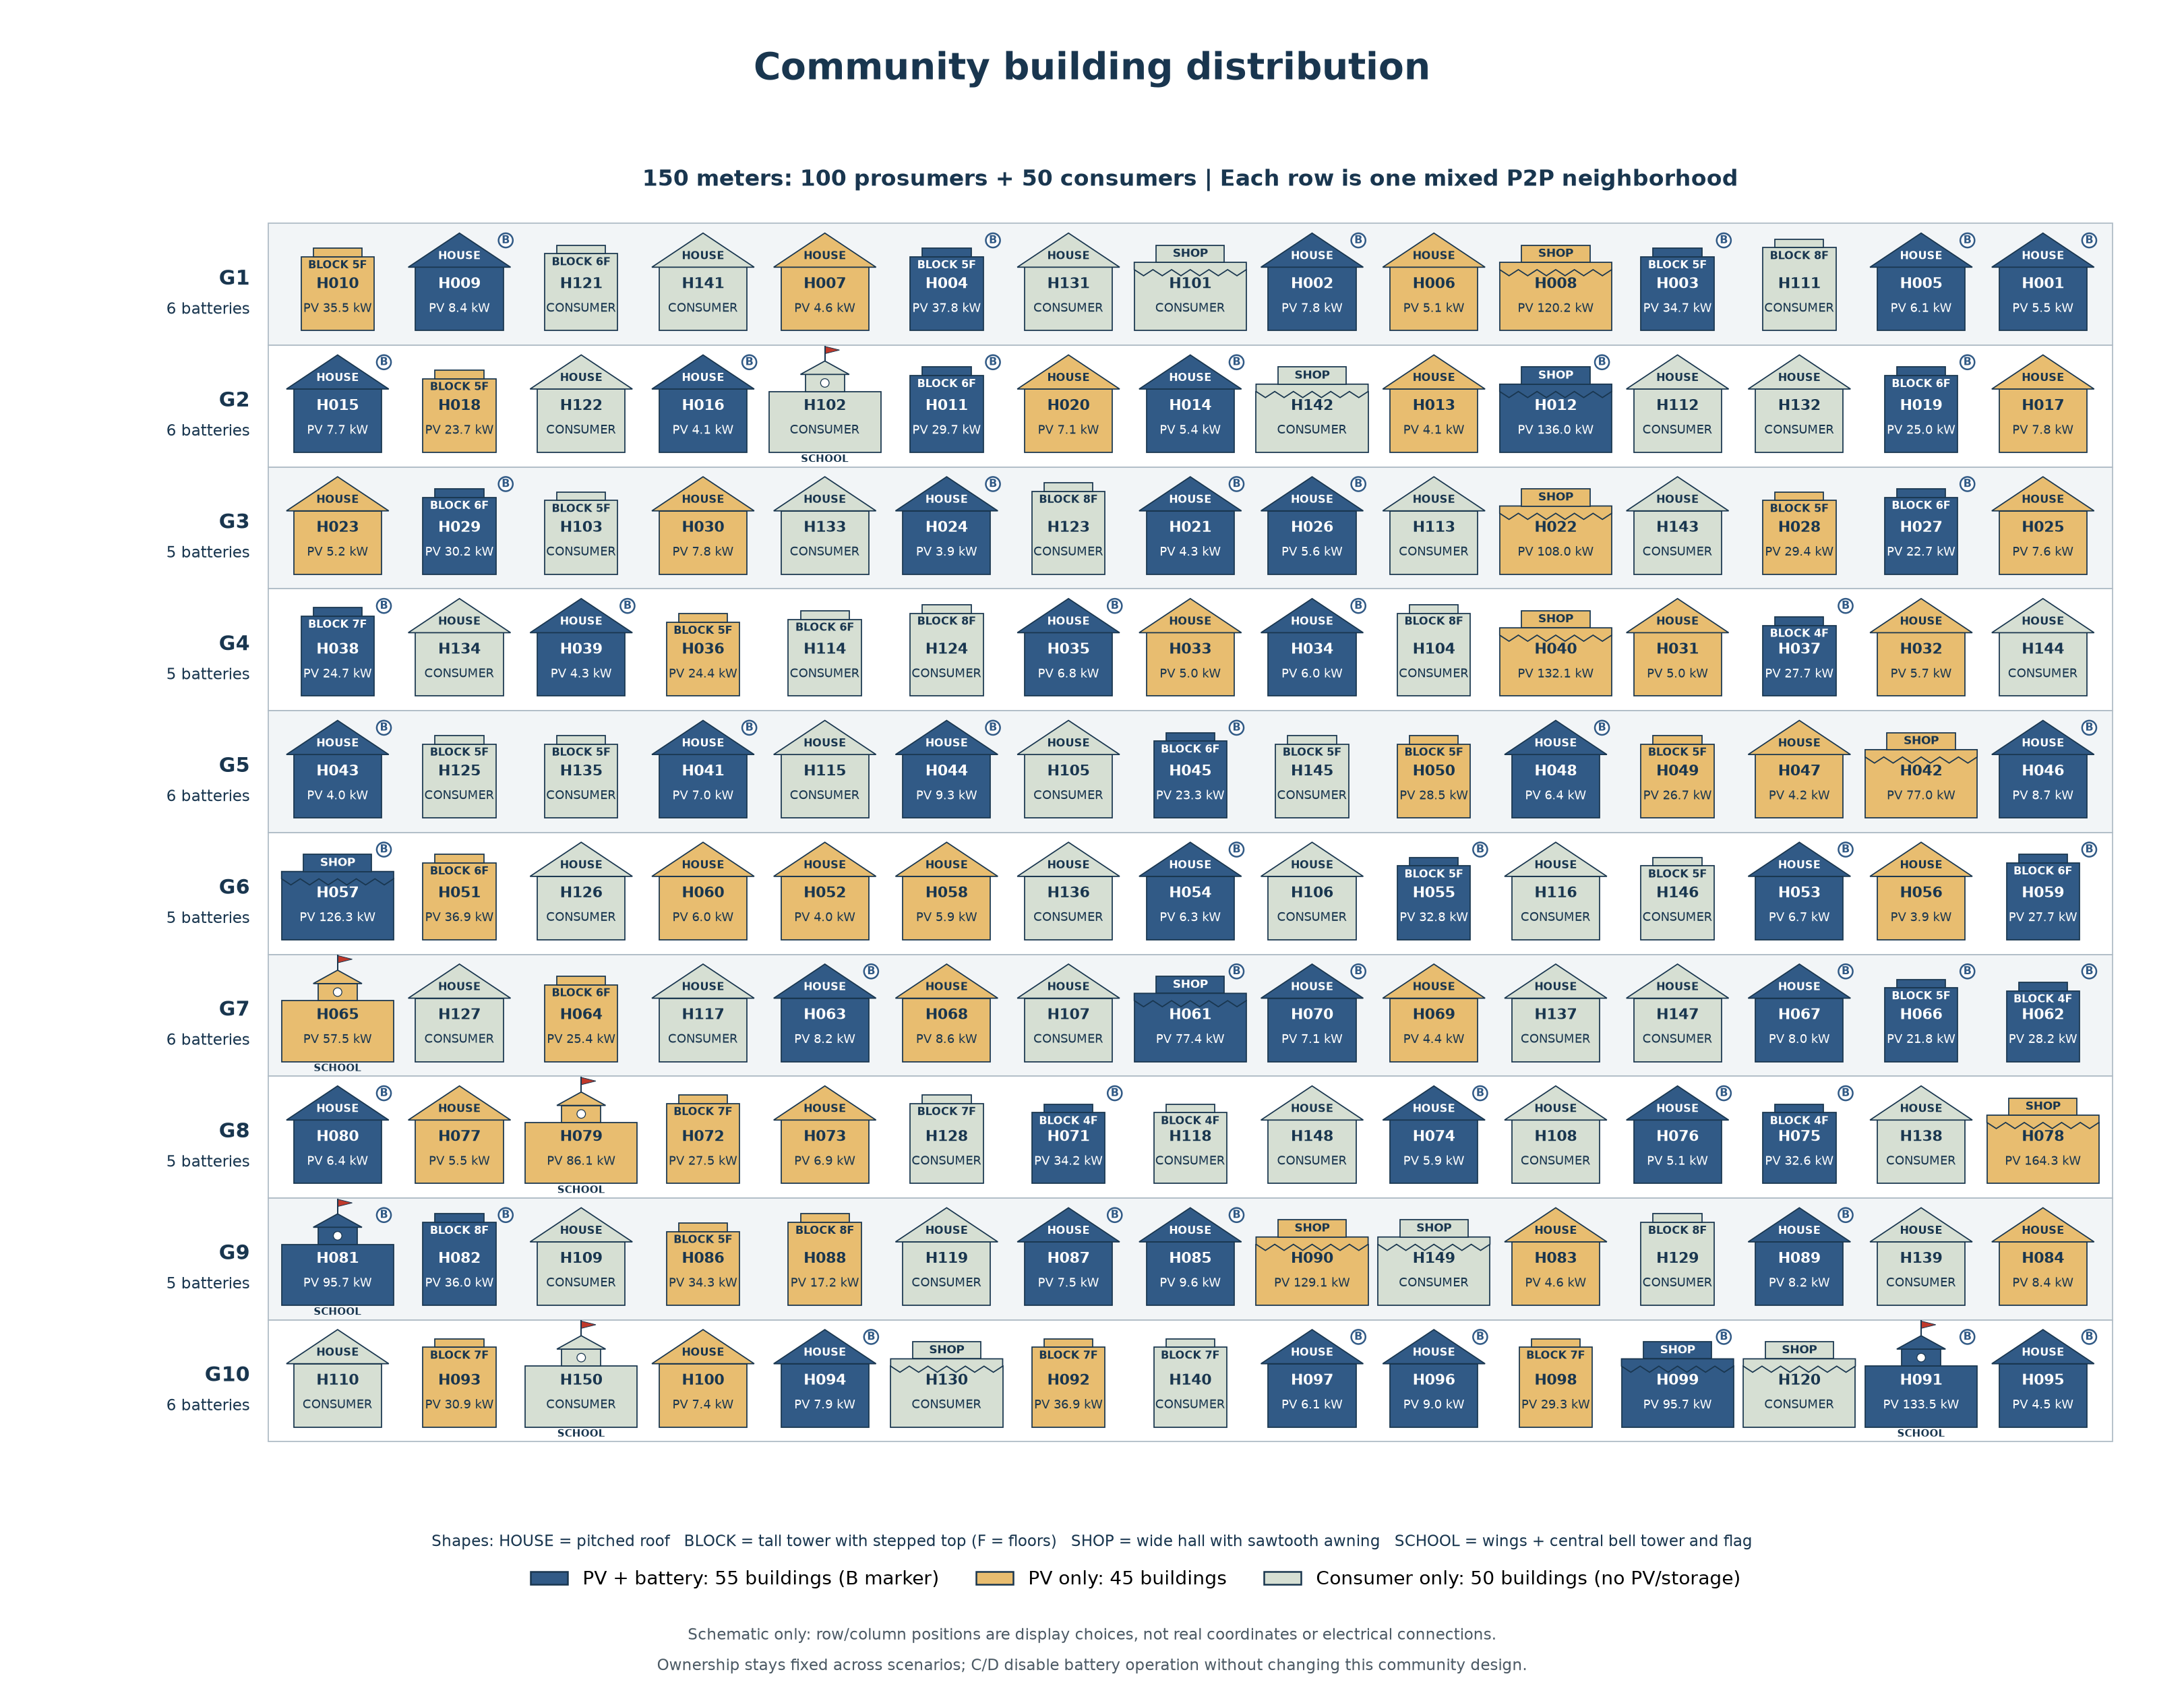
\includegraphics[width=\linewidth,height=0.45\textheight,keepaspectratio]{images/community_map.png}\end{center}

{\small Figure 1. Seeded community schematic: blue = PV + battery, gold = PV only, pale green and CONSUMER label = no PV/storage. Shapes show building type; F denotes floors. Display columns are shuffled independently of trading order. These are not geographic coordinates or feeder connections.\par}
\par\medskip

Every neighborhood has five or six battery owners. IDs, types and ownership stay fixed in all scenarios, including C/D where operation is disabled. The map is generated automatically by simulation runs with charts enabled, together with exact cell and group CSV exports.
\par\medskip

\clearpage

\section*{03  Building geometry and physical sizing}
\par\medskip

Type ranges are configurable in \textbf{config/buildings.py} and the buildings section of JSON. The following are proposed engineering defaults, not professor requirements or calibrated building-stock data.
\par\medskip

\begingroup\small
\begin{longtable}{>{\RaggedRight\arraybackslash}p{\dimexpr0.207101\linewidth-2\tabcolsep\relax}>{\RaggedRight\arraybackslash}p{\dimexpr0.082840\linewidth-2\tabcolsep\relax}>{\RaggedRight\arraybackslash}p{\dimexpr0.197239\linewidth-2\tabcolsep\relax}>{\RaggedRight\arraybackslash}p{\dimexpr0.118343\linewidth-2\tabcolsep\relax}>{\RaggedRight\arraybackslash}p{\dimexpr0.394477\linewidth-2\tabcolsep\relax}}
\toprule
\textbf{Type} & \textbf{Count} & \textbf{Single roof m2} & \textbf{Floors} & \textbf{Daily energy basis} \\ \midrule
\endfirsthead
\toprule
\textbf{Type} & \textbf{Count} & \textbf{Single roof m2} & \textbf{Floors} & \textbf{Daily energy basis} \\ \midrule
\endhead
Small house & 75 & 70-150 & 1-2 & 8-24 kWh per dwelling \\ \addlinespace[3pt]
Apartment block & 45 & 180-360 & 4-10 & 8-20 kWh per dwelling \\ \addlinespace[3pt]
Supermarket & 15 & 600-1400 & 1 & 0.5-1.1 kWh per m2 \\ \addlinespace[3pt]
School & 15 & 700-1600 & 2-3 & 0.08-0.18 kWh per m2 \\ \addlinespace[3pt]
\bottomrule
\end{longtable}
\endgroup

\subsection*{One roof, regardless of height}
\par\medskip

Total floor area = roof footprint x floors. Blocks contain 2-4 dwelling units per floor. Their demand basis scales with the total number of units. Commercial/school demand scales with total floor area. Small houses represent one dwelling even when they have two floors.
\par\medskip

\begin{lstlisting}
Prosumers: PV kW = min(roof m2 x usable share x density, type PV limit). Consumers: PV = 0; battery = none.
\end{lstlisting}

Usable roof fraction is 35-65\% and PV density is 0.20 kW/m2. Installed limits are 12 kW for houses, 100 kW for blocks, and 300 kW for supermarkets/schools. Floors and flats do not appear in the PV formula. Adding floors increases the demand basis without creating extra roof area.
\par\medskip

\subsection*{Actual seeded attributes, averaged per building}
\par\medskip

\begingroup\small
\begin{longtable}{>{\RaggedRight\arraybackslash}p{\dimexpr0.246548\linewidth-2\tabcolsep\relax}>{\RaggedRight\arraybackslash}p{\dimexpr0.177515\linewidth-2\tabcolsep\relax}>{\RaggedRight\arraybackslash}p{\dimexpr0.157791\linewidth-2\tabcolsep\relax}>{\RaggedRight\arraybackslash}p{\dimexpr0.216963\linewidth-2\tabcolsep\relax}>{\RaggedRight\arraybackslash}p{\dimexpr0.201183\linewidth-2\tabcolsep\relax}}
\toprule
\textbf{Type} & \textbf{Battery owners} & \textbf{Dwellings} & \textbf{Mean roof m2} & \textbf{Mean PV kW} \\ \midrule
\endfirsthead
\toprule
\textbf{Type} & \textbf{Battery owners} & \textbf{Dwellings} & \textbf{Mean roof m2} & \textbf{Mean PV kW} \\ \midrule
\endhead
Apartment block & 17 & 897 & 263.714 & 17.409 \\ \addlinespace[3pt]
School & 4 & 0 & 1,138.681 & 68.299 \\ \addlinespace[3pt]
Small house & 30 & 75 & 110.259 & 6.743 \\ \addlinespace[3pt]
Supermarket & 4 & 0 & 996.938 & 64.792 \\ \addlinespace[3pt]
\bottomrule
\end{longtable}
\endgroup

Battery capacity and charge/discharge power scale by type: 10 kWh / 3 kW for a house, 40 / 12 for a block, 100 / 30 for a supermarket and 60 / 18 for a school. Efficiency and SOC constraints remain identical. These scales can be overridden without changing ownership.
\par\medskip

\clearpage

\section*{04  Dynamic demand and solar forecasts}
\par\medskip

\begin{center}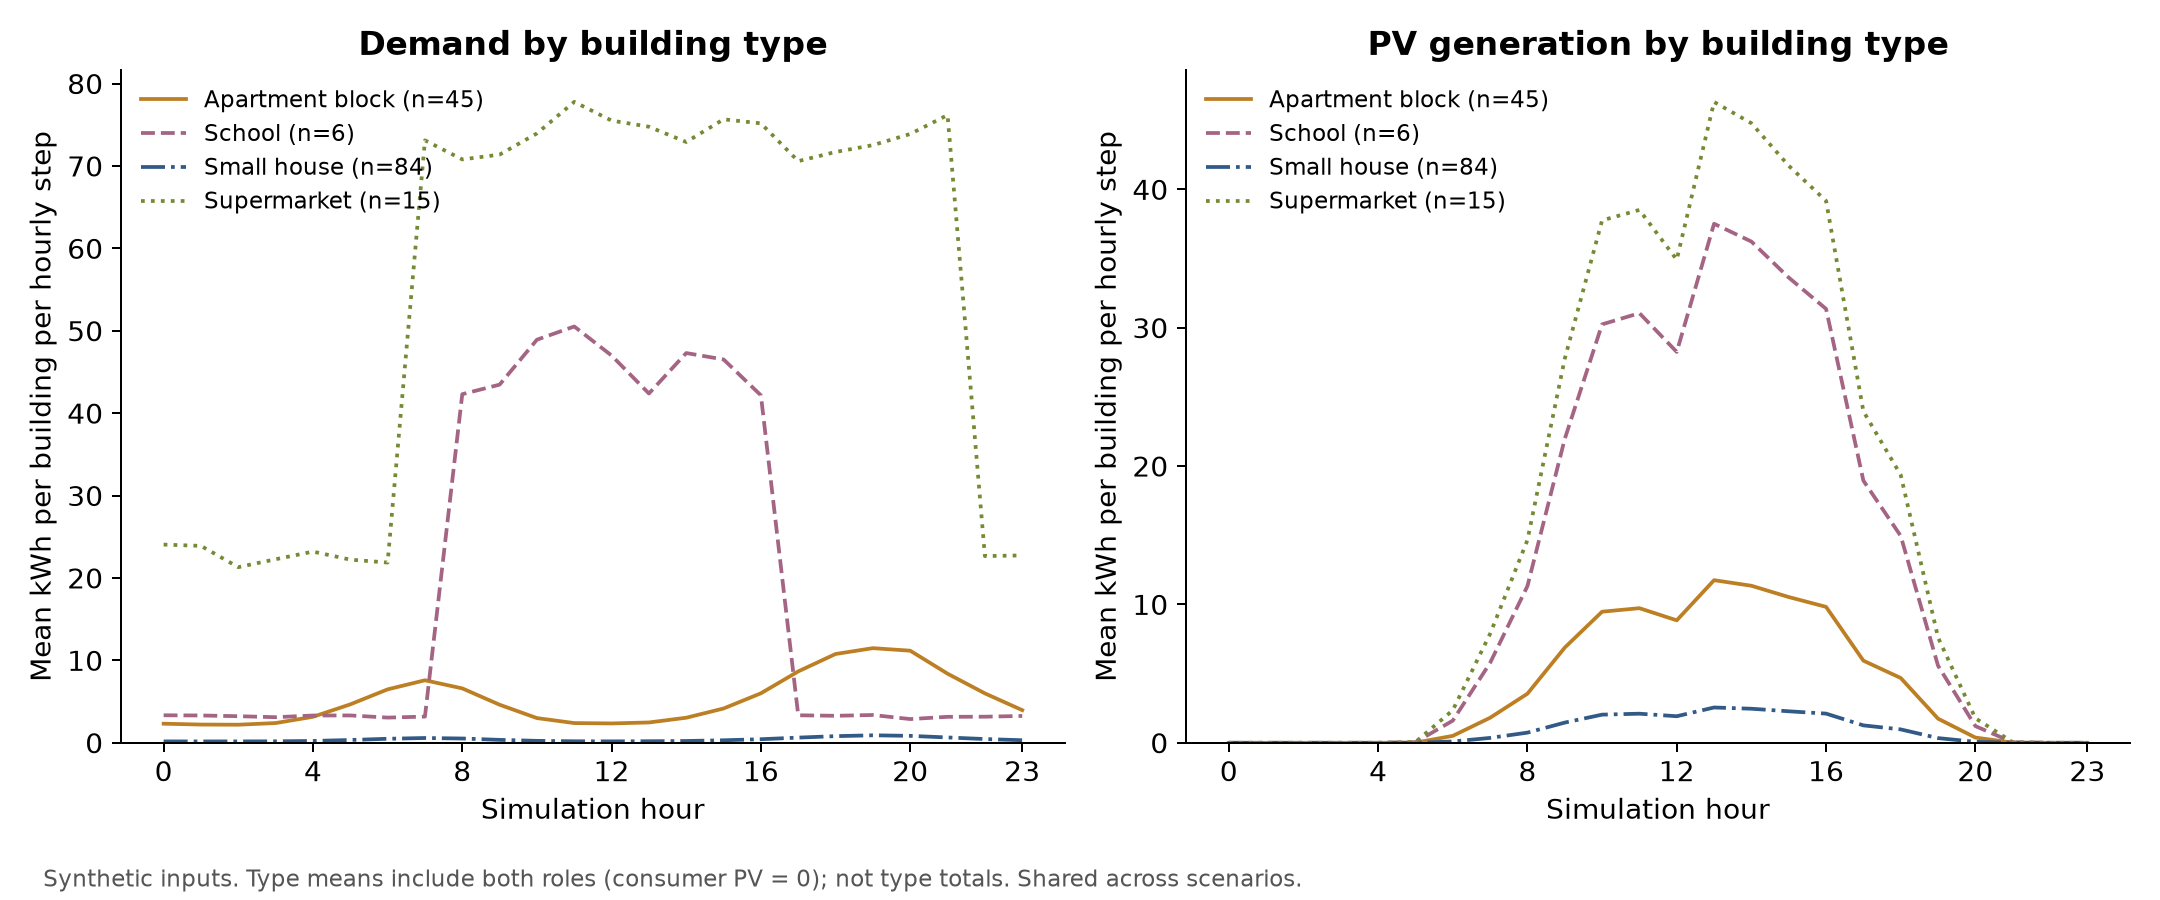
\includegraphics[width=\linewidth,height=0.45\textheight,keepaspectratio]{images/building_type_profiles.png}\end{center}

{\small Figure 2. Mean hourly energy per building type, including prosumers and consumers (whose PV is zero). These are not type totals. All scenarios reuse the same inputs; a lower mean PV than the old community does not mean original panels were removed.\par}
\par\medskip

\subsection*{Hourly activity and weekday/weekend behavior}
\par\medskip

Houses and blocks have morning/evening peaks with building-specific timing and hourly variation. Supermarkets retain a base load overnight and add operating load during 07:00-22:00. Schools operate during 08:00-17:00 on weekdays. Weekend daily energy is 105\% of weekday baseline for residential types, 90\% for supermarkets and 15\% for schools; school operating load is disabled on weekends.
\par\medskip

Each building receives a seeded daily multiplier within +/-8\%. Geometry stays fixed during the experiment; consumption changes by hour and date. A supplied aggregate demand CSV replaces this synthetic model. Weekends are modeled, but school terms, public holidays and weather-sensitive HVAC loads are not. Weekday school operation in June is an explicit simplification.
\par\medskip

\subsection*{PV and reference prices}
\par\medskip

PV kWh = installed kW x irradiance / 1000 x performance factor x hourly duration, capped at installed capacity. Nighttime production is zero. The default illustrative day starts 15 June 2026 at UTC+02:00, using a daylight curve and seeded cloud factors. Reference prices use only pre-start hourly observations; the default 14-day price history is synthetic. Forecast adapters reject missing coverage, duplicate keys and non-finite inputs.
\par\medskip

\clearpage

\section*{05  Trading, regulation and transaction record}
\par\medskip

\subsection*{Settlement sequence}
\par\medskip

\textbf{Self-balancing:} owner PV serves demand, with eligible battery operations. Consumers have demand only.\newline{}\textbf{P2P:} seeded buyer/seller encounters within each 15-member mixed group, at the seller ask.\newline{}\textbf{Aggregator:} lowest asks and highest bids across groups, at midpoint prices.\newline{}\textbf{External grid:} remaining demand imports at EUR 0.30/kWh and surplus exports at EUR 0.06/kWh. Consumers can buy but never supply electricity. Each trade updates remaining energy.
\par\medskip

\subsection*{Guidance and funded rewards}
\par\medskip

\begingroup\small
\begin{longtable}{>{\RaggedRight\arraybackslash}p{\dimexpr0.552268\linewidth-2\tabcolsep\relax}>{\RaggedRight\arraybackslash}p{\dimexpr0.447732\linewidth-2\tabcolsep\relax}}
\toprule
\textbf{Opening regulator funds} & \textbf{P2P seller reward} \\ \midrule
\endfirsthead
\toprule
\textbf{Opening regulator funds} & \textbf{P2P seller reward} \\ \midrule
\endhead
Below EUR 1 & EUR 0/kWh \\ \addlinespace[3pt]
EUR 1 to below EUR 5 & EUR 0.01/kWh \\ \addlinespace[3pt]
EUR 5 or above & EUR 0.02/kWh \\ \addlinespace[3pt]
\bottomrule
\end{longtable}
\endgroup

The fund starts at EUR 0. Guidance blends original offers toward 1.04 x reference for bids and 0.96 x reference for asks, with strength 0.65. Only P2P receives guidance. A full reward reservation is required before a discounted quote. Adjusted ask = guided ask - 50\% of reward rate. A successful seller receives trading payment plus full reward. Unaffordable quotes retry original offers without reward; rejected reservations are released.
\par\medskip

Regulated grid purchases and sales each pay EUR 0.01/kWh, collected after trading. New fees become available in the following hour. Opening funds fix that hour's reward tier. There are no internal fees or aggregator/grid seller rewards.
\par\medskip

\subsection*{Blockchain and conservation}
\par\medskip

Ten simulated miners take turns testing SHA-256 nonces inside one process. One block per hour records all completed P2P and aggregator trades exactly once. Each hash begins 000 and references its predecessor; the first references 64 zeros. Validation checks hashes, linkage, transaction contents and journal coverage. The blockchain does not choose energy quantities or prices.
\par\medskip

PV + discharge + purchases = demand + charge + sales.\newline{}Stored energy evolves as E\_next = E\_start + efficiency\_c x charge - discharge / efficiency\_d. Storage cannot charge and discharge simultaneously, charge from grid/P2P or sell stored energy.
\par\medskip

\clearpage

\section*{06  P2P results for the mixed community}
\par\medskip

\begin{center}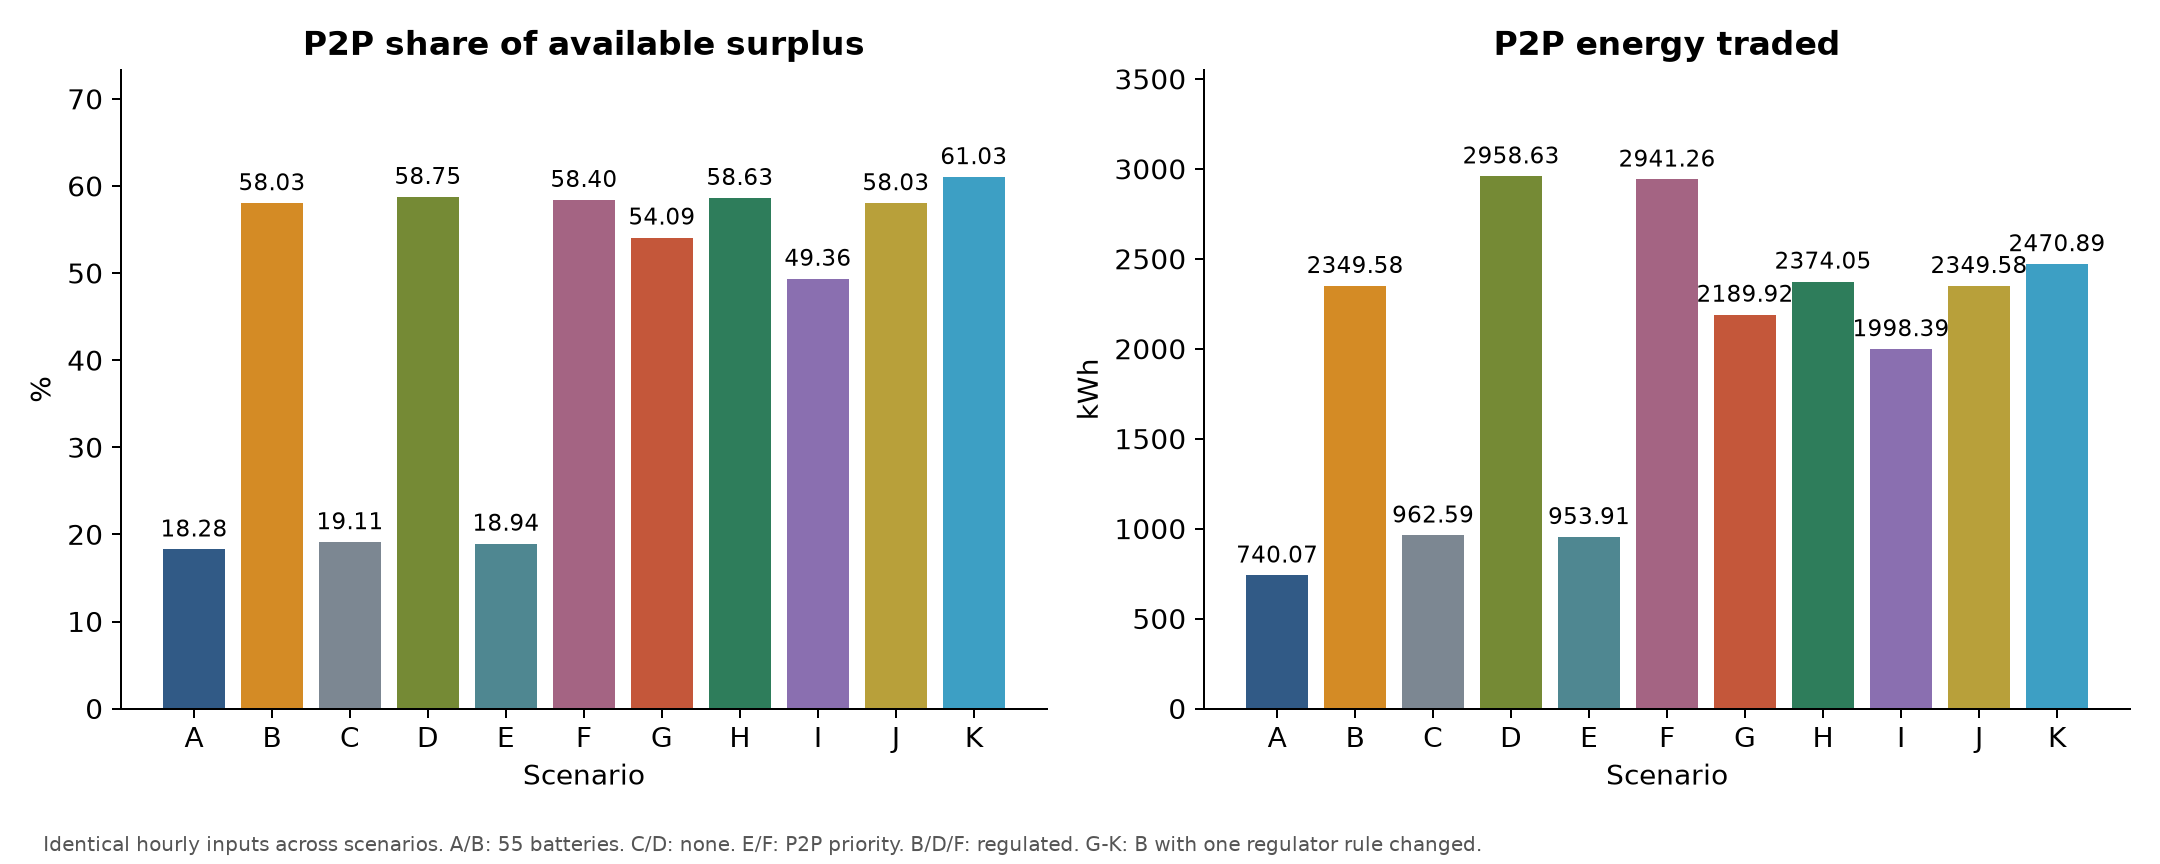
\includegraphics[width=\linewidth,height=0.45\textheight,keepaspectratio]{images/p2p_comparison.png}\end{center}

{\small Figure 3. Shared-input P2P outcomes. A/B use storage first; C/D disable it; E/F prioritize P2P before charging. B/D/F are regulated.\par}
\par\medskip

\begingroup\small
\begin{longtable}{>{\RaggedRight\arraybackslash}p{\dimexpr0.108481\linewidth-2\tabcolsep\relax}>{\RaggedRight\arraybackslash}p{\dimexpr0.187377\linewidth-2\tabcolsep\relax}>{\RaggedRight\arraybackslash}p{\dimexpr0.157791\linewidth-2\tabcolsep\relax}>{\RaggedRight\arraybackslash}p{\dimexpr0.355030\linewidth-2\tabcolsep\relax}>{\RaggedRight\arraybackslash}p{\dimexpr0.191321\linewidth-2\tabcolsep\relax}}
\toprule
\textbf{Scenario} & \textbf{P2P kWh} & \textbf{Share \%} & \textbf{Available surplus kWh} & \textbf{P2P trades} \\ \midrule
\endfirsthead
\toprule
\textbf{Scenario} & \textbf{P2P kWh} & \textbf{Share \%} & \textbf{Available surplus kWh} & \textbf{P2P trades} \\ \midrule
\endhead
A & 863.982 & 13.985 & 6,177.944 & 269 \\ \addlinespace[3pt]
B & 2,858.451 & 46.269 & 6,177.944 & 856 \\ \addlinespace[3pt]
C & 1,047.066 & 14.188 & 7,379.848 & 327 \\ \addlinespace[3pt]
D & 3,523.217 & 47.741 & 7,379.848 & 999 \\ \addlinespace[3pt]
E & 1,030.768 & 13.967 & 7,379.848 & 311 \\ \addlinespace[3pt]
F & 3,473.971 & 47.074 & 7,379.848 & 988 \\ \addlinespace[3pt]
\bottomrule
\end{longtable}
\endgroup

Primary KPI = 100 x P2P energy / surplus offered after self-balancing. In E/F the denominator includes PV subsequently stored after P2P, so compare absolute energy and raw PV surplus as well as shares. Zero denominators are undefined, not fabricated zeros.
\par\medskip

B minus A: P2P energy difference \textbf{+1994.469 kWh}.
\par\medskip

D minus C: P2P energy difference \textbf{+2476.151 kWh}.
\par\medskip

F minus E: P2P energy difference \textbf{+2443.203 kWh}.
\par\medskip

These differences describe the selected day and heuristic. Guidance cannot create surplus or demand, and no improvement is forced for other settings.
\par\medskip

\clearpage

\section*{07  Grid exchanges and financial results}
\par\medskip

\begin{center}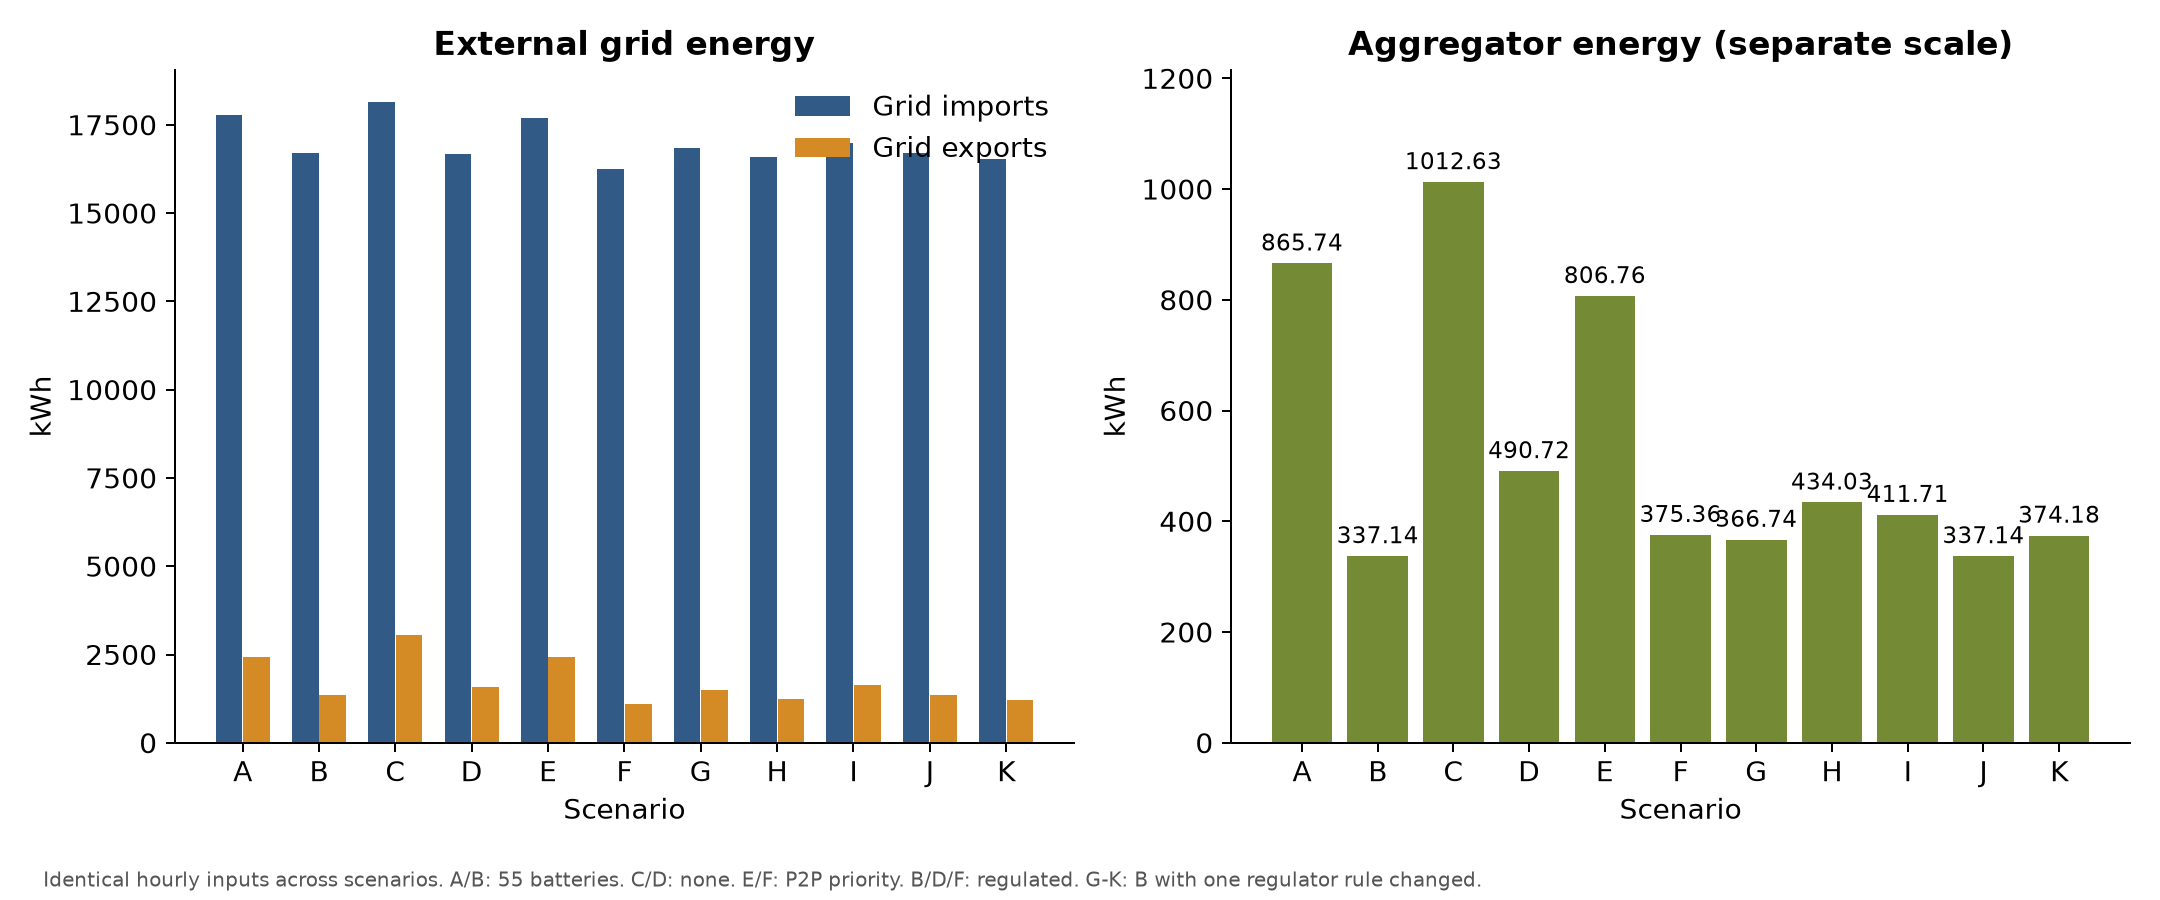
\includegraphics[width=\linewidth,height=0.45\textheight,keepaspectratio]{images/energy_comparison.png}\end{center}

{\small Figure 4. Grid settlement and aggregator energy use separate scales to retain visibility of internal volumes.\par}
\par\medskip

\begin{center}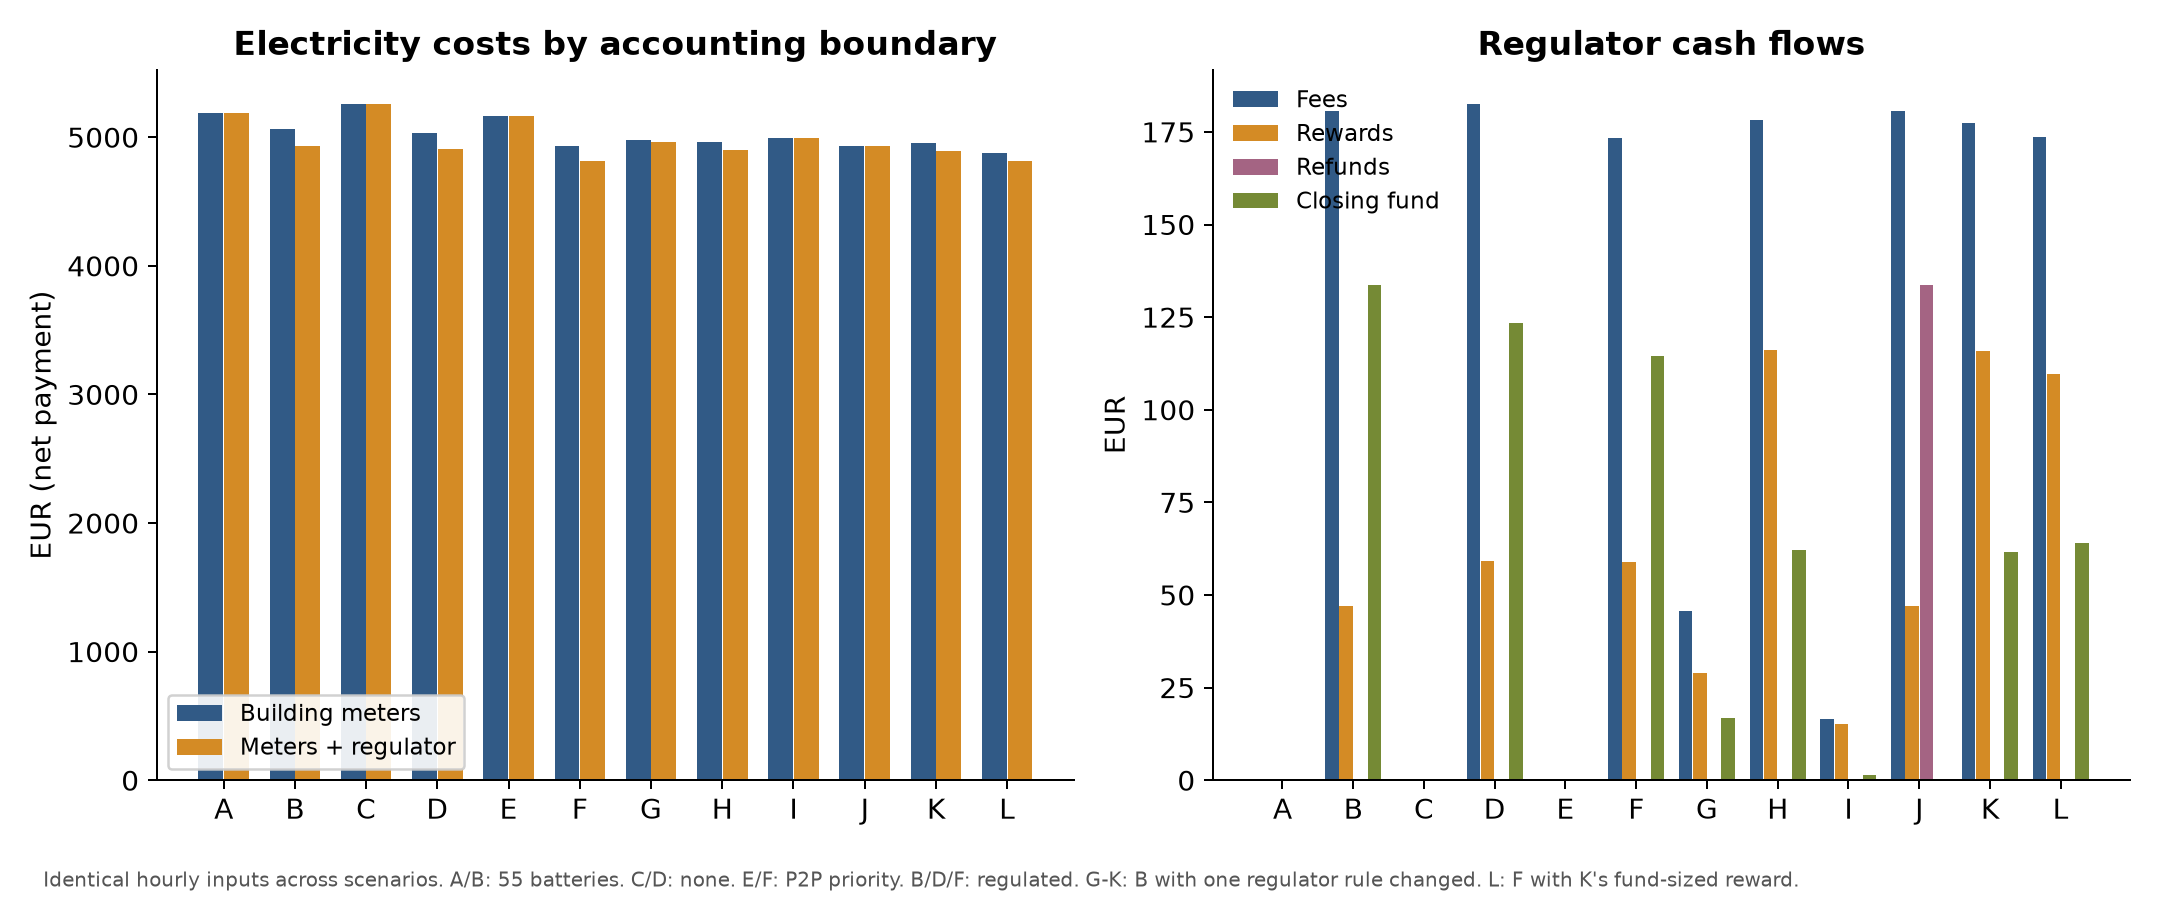
\includegraphics[width=\linewidth,height=0.45\textheight,keepaspectratio]{images/financial_comparison.png}\end{center}

{\small Figure 5. Building-meter net payments versus building meters plus the regulator, alongside fees, rewards and remaining funds.\par}
\par\medskip

Meter net cost = purchases - sale revenue + fees - rewards. Internal P2P/aggregator payments cancel over meters. Including the regulator subtracts the change in retained funds and equals net external-grid payments. Battery capital, aging, taxes and inventory valuation are excluded.
\par\medskip

A to B: meter cost EUR 5210.78 to 4978.98; meters plus regulator EUR 5210.78 to 4839.46. C to D: meter cost EUR 5382.51 to 5048.26. Cost effects need not have the same sign in every pair.
\par\medskip

\clearpage

\section*{08  Battery operation and available surplus}
\par\medskip

\begin{center}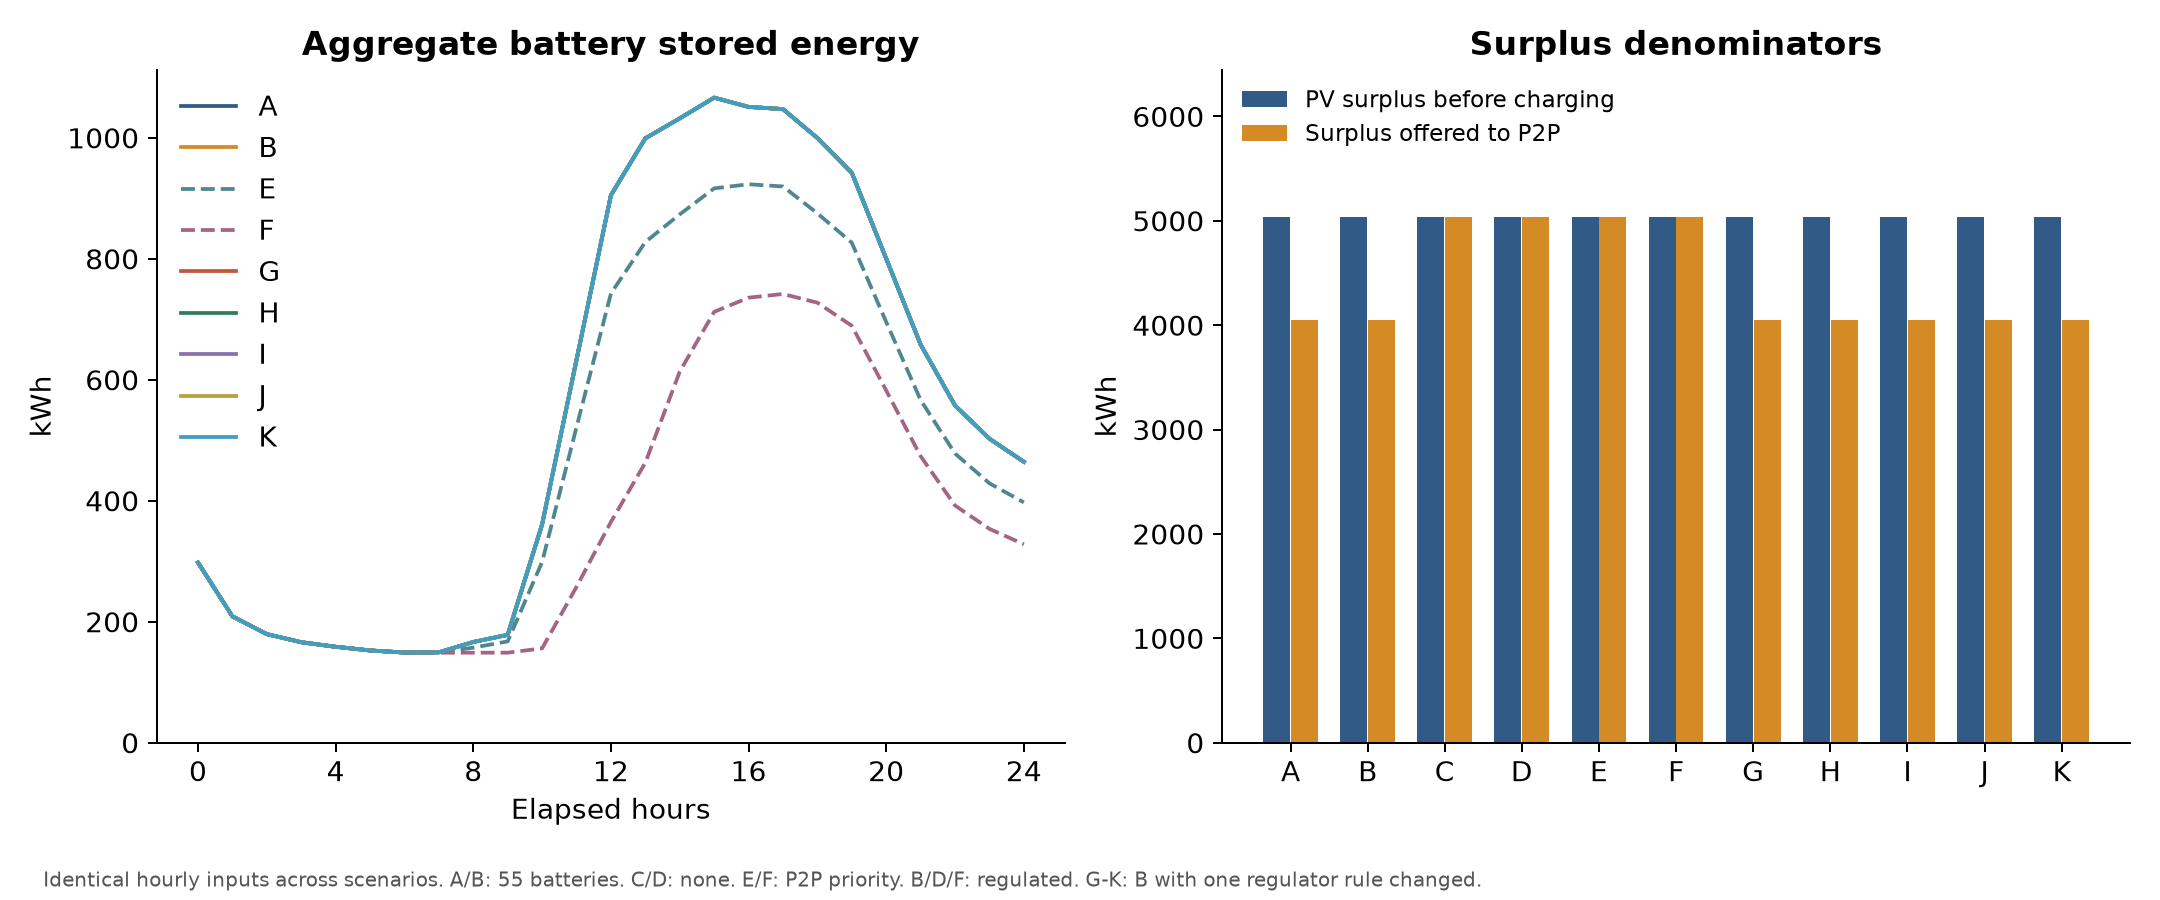
\includegraphics[width=\linewidth,height=0.45\textheight,keepaspectratio]{images/battery_and_surplus.png}\end{center}

{\small Figure 6. Aggregate storage and surplus denominators. A/B charge before P2P; E/F charge remaining PV after P2P. C/D have no active storage.\par}
\par\medskip

\begin{center}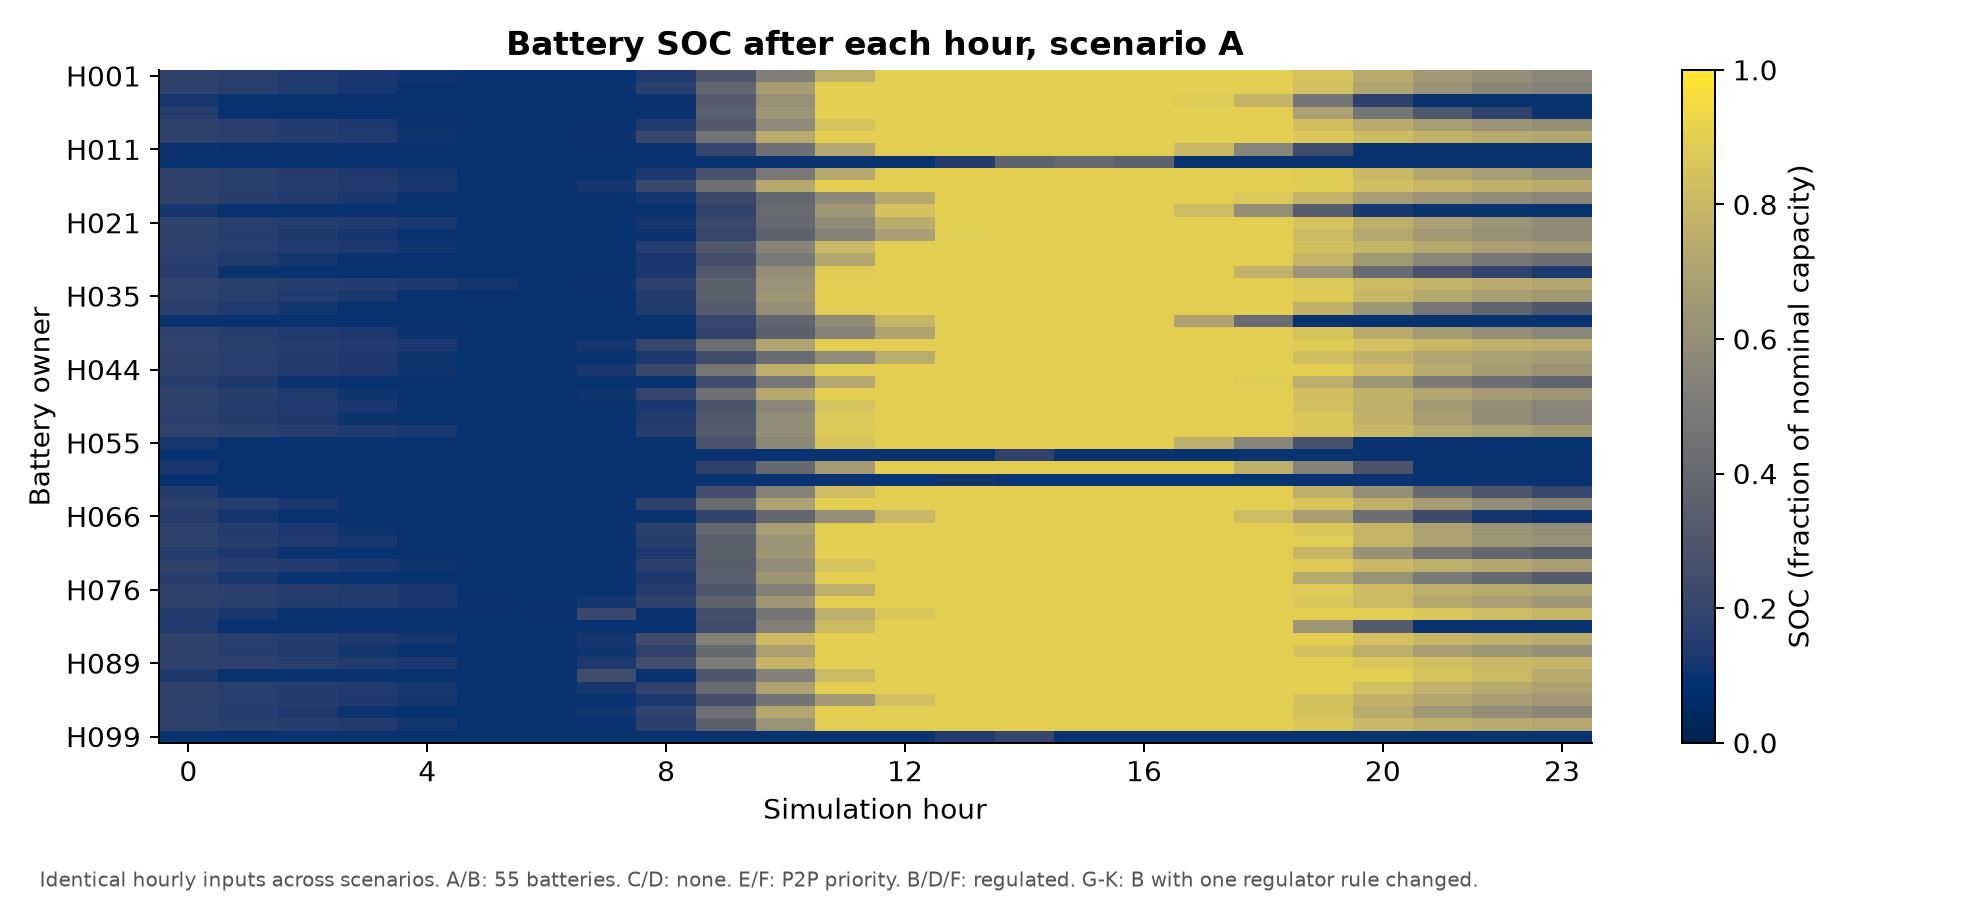
\includegraphics[width=\linewidth,height=0.45\textheight,keepaspectratio]{images/battery_soc.png}\end{center}

{\small Figure 7. End-of-hour SOC of the 55 owners in scenario A. Capacity and power differ by building type, while allowed SOC remains 10-90\%.\par}
\par\medskip

In A, AC charging is 1,201.904 kWh, discharge 1,018.134 kWh and conversion losses 113.681 kWh. Initial stored energy is 324.000 kWh and final storage 394.088 kWh. Initial inventory is exogenous; final inventory is reported without a monetary valuation.
\par\medskip

The global identity includes PV, demand, imports/exports, initial/final storage and explicit losses. It is checked independently of internal trading payments.
\par\medskip

\clearpage

\section*{09  Regulator budget and accounting boundary}
\par\medskip

\begin{center}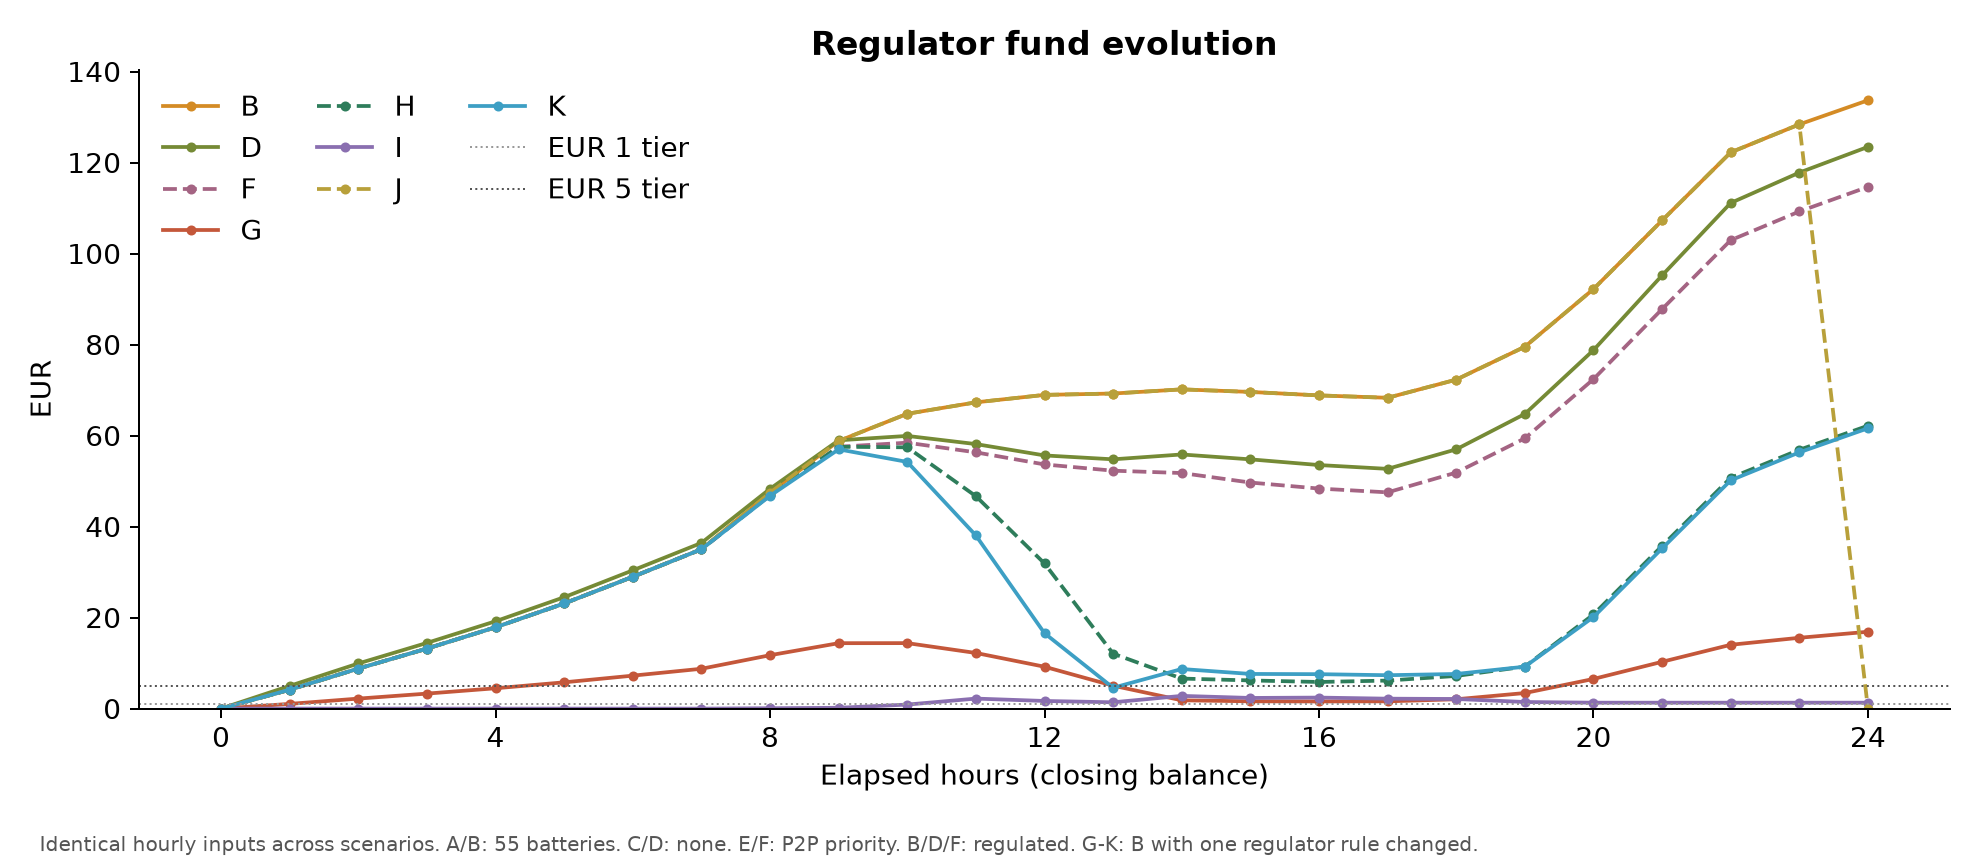
\includegraphics[width=\linewidth,height=0.45\textheight,keepaspectratio]{images/regulator_budget.png}\end{center}

{\small Figure 8. Closing funds across the day. An hour's opening balance selects the reward tier before that hour's new grid fees are collected.\par}
\par\medskip

\begingroup\small
\begin{longtable}{>{\RaggedRight\arraybackslash}p{\dimexpr0.128205\linewidth-2\tabcolsep\relax}>{\RaggedRight\arraybackslash}p{\dimexpr0.276134\linewidth-2\tabcolsep\relax}>{\RaggedRight\arraybackslash}p{\dimexpr0.276134\linewidth-2\tabcolsep\relax}>{\RaggedRight\arraybackslash}p{\dimexpr0.319527\linewidth-2\tabcolsep\relax}}
\toprule
\textbf{Scenario} & \textbf{Fees EUR} & \textbf{Rewards EUR} & \textbf{Closing fund EUR} \\ \midrule
\endfirsthead
\toprule
\textbf{Scenario} & \textbf{Fees EUR} & \textbf{Rewards EUR} & \textbf{Closing fund EUR} \\ \midrule
\endhead
B & 196.692 & 57.169 & 139.523 \\ \addlinespace[3pt]
D & 205.588 & 70.464 & 135.124 \\ \addlinespace[3pt]
F & 192.936 & 69.479 & 123.456 \\ \addlinespace[3pt]
\bottomrule
\end{longtable}
\endgroup

Closing fund = opening fund + grid fees - eligible P2P rewards. Every movement has a payer and payee. Reservations, releases, reward payments and hourly fund histories are exported. The ledger reconciles with the regulator's fund after each hour.
\par\medskip

Retained fees are a transfer from building meters to the regulator, not money destruction or an external resource cost. They can offset savings from better matching at the meter boundary. Accounts may pay for energy without a starting-cash restriction; only regulator guarantees are constrained by available funding.
\par\medskip

No end-of-day rebate is assumed. Changes to fees, reward tiers or guidance require a separately recorded configuration and rerun. The mixed-building outcomes cannot be attributed solely to regulation by comparing them with the old, physically different residential community.
\par\medskip

\clearpage

\section*{10  Verification, reproduction and limits}
\par\medskip

\subsection*{Recorded checks}
\par\medskip

The recorded full suite passed \textbf{85 tests} on 21 October 2026. All six saved scenarios passed independent energy, cash and blockchain verification. Tests include unchanged battery ownership, type allocation, one-roof sizing, increased block demand with floors, school weekend reduction, commercial night load, losses/SOC, rewards and forecast cutoff.
\par\medskip

Maximum absolute community energy residual: 3.64e-12 kWh. Maximum financial residual: 0 EUR. Numerical residuals are checked at explicit tolerances.
\par\medskip

\subsection*{Run and rebuild}
\par\medskip

\begin{lstlisting}
python -m pip install -r requirements.txt
python -m pytest -q
python main.py --include-priority
python scripts/verify_results.py
python -m pip install -r requirements-report.txt
python scripts/create_report.py
\end{lstlisting}

The simulator requires Python 3.11+ and was exercised on Python 3.14.7. PDF dependencies are optional. Use --config for JSON overrides, --output for separate experiment folders and --no-charts to skip visual exports. The historical residential model remains available through config/residential\_baseline.json.
\par\medskip

\subsection*{Scope and evidence}
\par\medskip

The model has no physical feeder limits, voltage/power-flow equations, land parcels, weather-sensitive HVAC, holiday/term calendar, battery aging or investment analysis. Hourly energy settlement and aggregate building meters are simplifying choices. A single synthetic day supports a demonstration, not a statistical or real-world performance claim. Presentations and ZIP packaging remain deferred.
\par\medskip

{\small Sources: supplied project brief and accepted building-meter revision; config/default.json; docs/building\_model.md; results/comparison.json and saved chart data; docs/current\_validation.json. The original residential comparison and report are preserved as a separate baseline.\par}
\par\medskip

{\small Input SHA-256: \texttt{\seqsplit{c42ebb8f3997ab181b6835907386d76365d642c4798b3b5b5a3752dd80e04e9b}}\par}
\par\medskip

\clearpage

\section*{11  Team guide: how to read the simulation}
\par\medskip

The next sections explain \textbf{all 166 configurable values} in the recorded experiment. Values come from scenario A's saved configuration in results/comparison.json, not from a possibly edited live JSON file. Other scenarios reuse the same base inputs and differ in their recorded storage/regulation switches.
\par\medskip

\begingroup\small
\begin{longtable}{>{\RaggedRight\arraybackslash}p{\dimexpr0.246548\linewidth-2\tabcolsep\relax}>{\RaggedRight\arraybackslash}p{\dimexpr0.753452\linewidth-2\tabcolsep\relax}}
\toprule
\textbf{Read first} & \textbf{Purpose} \\ \midrule
\endfirsthead
\toprule
\textbf{Read first} & \textbf{Purpose} \\ \midrule
\endhead
Pages 1-5 & Community, building types, physical models and trading rules. \\ \addlinespace[3pt]
Pages 6-10 & Actual outcomes and numerical verification. \\ \addlinespace[3pt]
Pages 12-20 and 22 & Exact parameter names, values, units and implemented effects. \\ \addlinespace[3pt]
Page 21 & Worked shared-roof example and steps for a controlled team experiment. \\ \addlinespace[3pt]
\bottomrule
\end{longtable}
\endgroup

\subsection*{Units and terms}
\par\medskip

\begingroup\small
\begin{longtable}{>{\RaggedRight\arraybackslash}p{\dimexpr0.246548\linewidth-2\tabcolsep\relax}>{\RaggedRight\arraybackslash}p{\dimexpr0.753452\linewidth-2\tabcolsep\relax}}
\toprule
\textbf{Term} & \textbf{What it means in this simulator} \\ \midrule
\endfirsthead
\toprule
\textbf{Term} & \textbf{What it means in this simulator} \\ \midrule
\endhead
kW & Power: an energy rate. A 3 kW charger can draw at most 3 kWh during one hour, before other limits. \\ \addlinespace[3pt]
kWh & Energy accumulated over a step or stored in a battery. Sum hourly energy to obtain a daily total. \\ \addlinespace[3pt]
EUR/kWh & Price per energy unit. Quantity x price gives the trading payment. EUR/MWh source data must be divided by 1000. \\ \addlinespace[3pt]
SOC & Stored energy / nominal battery capacity. 0.20 means 20\%, not 0.20 kWh. \\ \addlinespace[3pt]
Building / meter & One trading participant. A block aggregates its flats at one meter and shares one roof. \\ \addlinespace[3pt]
Dwelling unit & One residential flat/home inside a building. It is not automatically a separate P2P participant. \\ \addlinespace[3pt]
\bottomrule
\end{longtable}
\endgroup

\subsection*{Fixed properties versus dynamic values}
\par\medskip

Roof area, floors, flat count, PV capacity, offer factors and battery ownership are drawn once per experiment and stay fixed. Hourly PV, demand, SOC, trades, cash and regulator funds evolve through time. Shape weights redistribute a fixed daily energy baseline; they are not independently added kWh.
\par\medskip

Synthetic inputs and sizing ranges are teaching assumptions. A valid conservation check proves accounting consistency, not empirical realism or a guarantee of better economics.
\par\medskip

\clearpage

\section*{12  Parameters: community, time and randomness}
\par\medskip

JSON sections: simulation and buildings. Historical keys containing household now count building meters in the mixed model. A report value is not applied to new runs until it is saved in the chosen configuration.
\par\medskip

\begingroup\small
\begin{longtable}{>{\RaggedRight\arraybackslash}p{\dimexpr0.285996\linewidth-2\tabcolsep\relax}>{\RaggedRight\arraybackslash}p{\dimexpr0.207101\linewidth-2\tabcolsep\relax}>{\RaggedRight\arraybackslash}p{\dimexpr0.506903\linewidth-2\tabcolsep\relax}}
\toprule
\textbf{Exact JSON key} & \textbf{Value used / units} & \textbf{Meaning and effect of changing it} \\ \midrule
\endfirsthead
\toprule
\textbf{Exact JSON key} & \textbf{Value used / units} & \textbf{Meaning and effect of changing it} \\ \midrule
\endhead
simulation.\allowbreak{}household\_\allowbreak{}count & 100 (prosumer meters) & Number of original PV-equipped aggregate meters, not flats.\allowbreak{} Consumer-only additions are configured separately.\allowbreak{} Must divide evenly into group\_\allowbreak{}count.\allowbreak{} \\ \addlinespace[3pt]
simulation.\allowbreak{}group\_\allowbreak{}count & 10 (groups) & Number of P2P neighborhoods. Group size = (prosumers + consumers) / group count. Changes which meters can trade directly. \\ \addlinespace[3pt]
simulation.\allowbreak{}battery\_\allowbreak{}household\_\allowbreak{}count & 55 (owners) & Exact number of battery-owning meters. IDs are selected with the seed and spread evenly across groups. C/D disable operation, not ownership. \\ \addlinespace[3pt]
simulation.hours & 24 (one-hour steps) & Length of the run. 24 covers one day; 168 covers a week and exposes weekend effects. Longer runs do not add holiday logic. \\ \addlinespace[3pt]
simulation.\allowbreak{}timestep\_\allowbreak{}hours & 1 (hours per step) & This implementation supports exactly 1. Do not change it to 0.5: the hourly input generator rejects other durations. \\ \addlinespace[3pt]
simulation.\allowbreak{}random\_\allowbreak{}seed & 42 (integer) & Controls randomized ownership, type positions, building attributes, cloud factors, demand variation and encounter order through separate seeded streams. \\ \addlinespace[3pt]
simulation.\allowbreak{}log\_\allowbreak{}level & INFO (logging level) & Console verbosity: DEBUG, INFO, WARNING, ERROR or CRITICAL. Does not change energy or prices. \\ \addlinespace[3pt]
buildings.enabled & true (boolean) & true selects the mixed-building model. false selects the original individual-house model; type geometry and type battery scales are then unused. \\ \addlinespace[3pt]
buildings.\allowbreak{}consumer\_\allowbreak{}count & 50 (additional meters) & Extra consumer-only buildings with zero PV and no battery.\allowbreak{} Types follow the same shares; additions split equally across groups.\allowbreak{} Total meters = household\_\allowbreak{}count + consumer\_\allowbreak{}count.\allowbreak{} \\ \addlinespace[3pt]
buildings.\allowbreak{}pv\_\allowbreak{}density\_\allowbreak{}kw\_\allowbreak{}m2 & 0.2 (kW per usable m2) & Installed PV power per usable roof area. Higher density raises capacity until the type PV limit is reached. It does not multiply roof area by floors. \\ \addlinespace[3pt]
\bottomrule
\end{longtable}
\endgroup

Constraints: equal neighborhood sizes; battery owners between zero and meter count; positive duration; currently one-hour steps only. Shares are rounded separately within each group, so small custom groups may not reproduce exact requested type percentages.
\par\medskip

The seed is held fixed across scenarios. Changing it creates a different realization and should be recorded as a new experiment, rather than interpreted as the effect of one policy switch.
\par\medskip

\clearpage

\section*{13  Parameters: building geometry and composition}
\par\medskip

Prefix: buildings.types.<type>., where type is small\_house, apartment\_block, supermarket or school. Values apply to both roles. H001-H100 are original prosumers; H101-H150 are added consumers with no PV or battery, regardless of roof potential.
\par\medskip

\begingroup\small
\begin{longtable}{>{\RaggedRight\arraybackslash}p{\dimexpr0.228797\linewidth-2\tabcolsep\relax}>{\RaggedRight\arraybackslash}p{\dimexpr0.074951\linewidth-2\tabcolsep\relax}>{\RaggedRight\arraybackslash}p{\dimexpr0.074951\linewidth-2\tabcolsep\relax}>{\RaggedRight\arraybackslash}p{\dimexpr0.088757\linewidth-2\tabcolsep\relax}>{\RaggedRight\arraybackslash}p{\dimexpr0.084813\linewidth-2\tabcolsep\relax}>{\RaggedRight\arraybackslash}p{\dimexpr0.447732\linewidth-2\tabcolsep\relax}}
\toprule
\textbf{Key under each type} & \textbf{House} & \textbf{Block} & \textbf{Market} & \textbf{School} & \textbf{Units and meaning} \\ \midrule
\endfirsthead
\toprule
\textbf{Key under each type} & \textbf{House} & \textbf{Block} & \textbf{Market} & \textbf{School} & \textbf{Units and meaning} \\ \midrule
\endhead
share & 0.5 & 0.3 & 0.1 & 0.1 & fraction. Type fraction; four shares sum to 1. Prosumers round within each group; consumers round across their full pool, then shuffle into equal group additions. \\ \addlinespace[3pt]
roof\_\allowbreak{}min\_\allowbreak{}m2 & 70 & 180 & 600 & 700 & m2. Lower bound of the sampled single roof footprint; higher area permits more PV and increases the area-based commercial/school load basis. \\ \addlinespace[3pt]
roof\_\allowbreak{}max\_\allowbreak{}m2 & 150 & 360 & 1400 & 1600 & m2. Upper bound of that roof draw. One roof per building, regardless of floor count. \\ \addlinespace[3pt]
floors\_\allowbreak{}min & 1 & 4 & 1 & 2 & floors. Lower bound of the integer floor draw. Raises block dwelling counts and school floor area, without adding PV roofs. \\ \addlinespace[3pt]
floors\_\allowbreak{}max & 2 & 10 & 1 & 3 & floors. Upper floor-count bound. Total floor area = roof footprint x sampled floors. \\ \addlinespace[3pt]
units\_\allowbreak{}per\_\allowbreak{}floor\_\allowbreak{}min & 1 & 2 & 1 & 1 & flats per floor. Lower integer bound, used to calculate block flats. Small houses always have one dwelling; schools/shops have zero residential dwellings. \\ \addlinespace[3pt]
units\_\allowbreak{}per\_\allowbreak{}floor\_\allowbreak{}max & 1 & 4 & 1 & 1 & flats per floor. Upper bound for block flats per floor. More flats increase aggregate residential demand, not roof size. \\ \addlinespace[3pt]
roof\_\allowbreak{}usable\_\allowbreak{}fraction\_\allowbreak{}min & 0.35 & 0.35 & 0.35 & 0.35 & fraction. Lower bound of the usable roof share for PV. Excludes the rest of the roof from installed-panel area. \\ \addlinespace[3pt]
roof\_\allowbreak{}usable\_\allowbreak{}fraction\_\allowbreak{}max & 0.65 & 0.65 & 0.65 & 0.65 & fraction.\allowbreak{} Upper usable-share bound.\allowbreak{} Capacity = min(roof x usable share x density, pv\_\allowbreak{}limit\_\allowbreak{}kw).\allowbreak{} \\ \addlinespace[3pt]
pv\_\allowbreak{}limit\_\allowbreak{}kw & 12 & 100 & 300 & 300 & kW. Upper installed-PV limit for one building. Raising it matters only where the roof-based capacity would exceed the old limit. \\ \addlinespace[3pt]
battery\_\allowbreak{}scale & 1 & 4 & 10 & 6 & multiplier. For owners, multiplies base storage capacity and both power limits. Does not change owner count, SOC fractions or efficiency. \\ \addlinespace[3pt]
\bottomrule
\end{longtable}
\endgroup

Roof and floor area are different quantities. Type PV limits constrain the single roof; floors never create duplicate roofs. Battery scale changes equipment sizes only for existing owners, preserving the selected 55 owner IDs in this run.
\par\medskip

\clearpage

\section*{14  Parameters: building demand and schedules}
\par\medskip

Prefix: buildings.types.<type>. Daily energy is drawn first, then distributed over 24 hours. The realized total may differ after weekend and per-date variation. Operating hours use the configured fixed local offset.
\par\medskip

\begingroup\small
\begin{longtable}{>{\RaggedRight\arraybackslash}p{\dimexpr0.228797\linewidth-2\tabcolsep\relax}>{\RaggedRight\arraybackslash}p{\dimexpr0.074951\linewidth-2\tabcolsep\relax}>{\RaggedRight\arraybackslash}p{\dimexpr0.074951\linewidth-2\tabcolsep\relax}>{\RaggedRight\arraybackslash}p{\dimexpr0.088757\linewidth-2\tabcolsep\relax}>{\RaggedRight\arraybackslash}p{\dimexpr0.084813\linewidth-2\tabcolsep\relax}>{\RaggedRight\arraybackslash}p{\dimexpr0.447732\linewidth-2\tabcolsep\relax}}
\toprule
\textbf{Key under each type} & \textbf{House} & \textbf{Block} & \textbf{Market} & \textbf{School} & \textbf{Units and meaning} \\ \midrule
\endfirsthead
\toprule
\textbf{Key under each type} & \textbf{House} & \textbf{Block} & \textbf{Market} & \textbf{School} & \textbf{Units and meaning} \\ \midrule
\endhead
daily\_\allowbreak{}energy\_\allowbreak{}min & 8 & 8 & 0.5 & 0.08 & basis-dependent.\allowbreak{} Lower base energy draw: kWh/dwelling/day for per\_\allowbreak{}dwelling, or kWh/m2/day for per\_\allowbreak{}floor\_\allowbreak{}area.\allowbreak{} Before weekend/day multipliers.\allowbreak{} \\ \addlinespace[3pt]
daily\_\allowbreak{}energy\_\allowbreak{}max & 24 & 20 & 1.1 & 0.18 & basis-dependent. Upper energy draw. Multiply by dwelling count or total floor area to obtain the building weekday daily baseline. \\ \addlinespace[3pt]
energy\_\allowbreak{}basis & per\_\allowbreak{}dwelling & per\_\allowbreak{}dwelling & per\_\allowbreak{}floor\_\allowbreak{}area & per\_\allowbreak{}floor\_\allowbreak{}area & enum.\allowbreak{} per\_\allowbreak{}dwelling uses dwelling count; per\_\allowbreak{}floor\_\allowbreak{}area uses roof x floors.\allowbreak{} Keep houses/blocks on dwelling basis and nonresidential buildings on area basis.\allowbreak{} \\ \addlinespace[3pt]
profile & residential & residential & commercial & school & enum. residential uses morning/evening peaks. commercial and school use a base plus an opening-hour load. Type name alone does not override this field. \\ \addlinespace[3pt]
opening\_\allowbreak{}hour & 7 & 7 & 7 & 8 & local hour. Start of operating activity, inclusive. Used by nonresidential profiles; ignored by residential profiles. \\ \addlinespace[3pt]
closing\_\allowbreak{}hour & 22 & 22 & 22 & 17 & local hour. End of operating activity, exclusive. A school closing at 17 has no operating component in the 17:00-18:00 step. \\ \addlinespace[3pt]
base\_\allowbreak{}load\_\allowbreak{}weight & 0.25 & 0.25 & 0.45 & 0.08 & relative weight. Positive all-hour load weight. It sets profile shape relative to peaks/operation; hourly weights are normalized to the daily energy, so this is not a kW value. \\ \addlinespace[3pt]
operating\_\allowbreak{}load\_\allowbreak{}weight & 1 & 1 & 1 & 1 & relative weight. Additional weight while operating. Used by commercial/school profiles; ignored by residential profiles. Changes hourly distribution, not the daily baseline total. \\ \addlinespace[3pt]
weekend\_\allowbreak{}multiplier & 1.05 & 1.05 & 0.9 & 0.15 & fraction/multiplier. Saturday/Sunday daily energy relative to the weekday baseline. 0.15 means 15\%, not a 15\% reduction. Daily random variation still applies. \\ \addlinespace[3pt]
weekend\_\allowbreak{}open & true & true & true & false & boolean. Whether the nonresidential operating component remains active on weekends. false removes operating activity but does not remove the base load. \\ \addlinespace[3pt]
daily\_\allowbreak{}variation\_\allowbreak{}fraction & 0.08 & 0.08 & 0.08 & 0.08 & fraction. Seeded per-building, per-date variation. 0.08 samples a multiplier between 0.92 and 1.08, shared by all hours of that building's day. \\ \addlinespace[3pt]
\bottomrule
\end{longtable}
\endgroup

Example: a school's weekday baseline of 400 kWh becomes a 60 kWh weekend baseline at multiplier 0.15, then receives its seeded daily factor. This is an illustration of the rule, not an observed or reported school measurement.
\par\medskip

\clearpage

\section*{15  Parameters: batteries and energy losses}
\par\medskip

Prefix: simulation.battery. Type battery\_scale multiplies the three sizing values; fractions and strategy are not scaled. Storage cannot use purchased electricity or discharge beyond owner demand.
\par\medskip

\begingroup\small
\begin{longtable}{>{\RaggedRight\arraybackslash}p{\dimexpr0.285996\linewidth-2\tabcolsep\relax}>{\RaggedRight\arraybackslash}p{\dimexpr0.207101\linewidth-2\tabcolsep\relax}>{\RaggedRight\arraybackslash}p{\dimexpr0.506903\linewidth-2\tabcolsep\relax}}
\toprule
\textbf{Exact JSON key} & \textbf{Value used / units} & \textbf{Meaning and effect of changing it} \\ \midrule
\endfirsthead
\toprule
\textbf{Exact JSON key} & \textbf{Value used / units} & \textbf{Meaning and effect of changing it} \\ \midrule
\endhead
simulation.\allowbreak{}battery.\allowbreak{}capacity\_\allowbreak{}kwh & 10 (kWh) & Base nominal stored-energy capacity.\allowbreak{} Each owning building multiplies this by its battery\_\allowbreak{}scale.\allowbreak{} \\ \addlinespace[3pt]
simulation.\allowbreak{}battery.\allowbreak{}max\_\allowbreak{}charge\_\allowbreak{}power\_\allowbreak{}kw & 3 (kW) & Base AC charging power limit. Maximum step energy = scaled power x hours, also limited by PV surplus and SOC headroom. \\ \addlinespace[3pt]
simulation.\allowbreak{}battery.\allowbreak{}max\_\allowbreak{}discharge\_\allowbreak{}power\_\allowbreak{}kw & 3 (kW) & Base AC power delivered from storage. Also limited by owner demand and stored energy above minimum SOC. \\ \addlinespace[3pt]
simulation.\allowbreak{}battery.\allowbreak{}charge\_\allowbreak{}efficiency & 0.95 (fraction) & Fraction of AC charging energy retained in storage. 0.95 stores 0.95 kWh for every 1 kWh entering; the remainder is a loss. \\ \addlinespace[3pt]
simulation.\allowbreak{}battery.\allowbreak{}discharge\_\allowbreak{}efficiency & 0.95 (fraction) & Fraction of removed stored energy delivered to demand. Delivering 1 kWh removes 1 / efficiency kWh from storage. \\ \addlinespace[3pt]
simulation.\allowbreak{}battery.\allowbreak{}initial\_\allowbreak{}soc & 0.2 (fraction of capacity) & Starting inventory, not a charging transaction. 0.20 starts at 20\% of each building's scaled nominal capacity. \\ \addlinespace[3pt]
simulation.\allowbreak{}battery.\allowbreak{}min\_\allowbreak{}soc & 0.1 (fraction of capacity) & Lower stored-energy reserve. Raising it reduces energy available for discharge. \\ \addlinespace[3pt]
simulation.\allowbreak{}battery.\allowbreak{}max\_\allowbreak{}soc & 0.9 (fraction of capacity) & Upper stored-energy bound. Lowering it reduces charging room. min <= initial <= max is required. \\ \addlinespace[3pt]
simulation.battery.strategy & self\_\allowbreak{}consumption\_\allowbreak{}first (enum) & Engine default: self\_\allowbreak{}consumption\_\allowbreak{}first or p2p\_\allowbreak{}priority.\allowbreak{} Named experiments override it: A/B select the first; E/F select the second.\allowbreak{} C/D disable storage.\allowbreak{} \\ \addlinespace[3pt]
\bottomrule
\end{longtable}
\endgroup

Equipment multipliers used: small\_house: x1, apartment\_block: x4, supermarket: x10, school: x6. Min/initial/max SOC must be ordered and efficiencies must lie in (0,1]. Named A-F scenarios override the engine strategy field as shown on section 1.
\par\medskip

\subsection*{Worked AC-side example}
\par\medskip

If headroom and surplus allow a 3 kWh charge, storage gains 2.850 kWh and loses 0.150 kWh. Delivering 1 kWh to demand removes 1.0526 kWh from storage, with 0.0526 kWh lost. Power and SOC limits may reduce these illustrative quantities.
\par\medskip

\clearpage

\section*{16  Parameters: weather, prices and input files}
\par\medskip

Prefix: forecast. CSV paths replace only the corresponding synthetic input. null means use the fallback. All input types remain explicitly labeled in hourly\_inputs.csv.
\par\medskip

\begingroup\small
\begin{longtable}{>{\RaggedRight\arraybackslash}p{\dimexpr0.285996\linewidth-2\tabcolsep\relax}>{\RaggedRight\arraybackslash}p{\dimexpr0.207101\linewidth-2\tabcolsep\relax}>{\RaggedRight\arraybackslash}p{\dimexpr0.506903\linewidth-2\tabcolsep\relax}}
\toprule
\textbf{Exact JSON key} & \textbf{Value used / units} & \textbf{Meaning and effect of changing it} \\ \midrule
\endfirsthead
\toprule
\textbf{Exact JSON key} & \textbf{Value used / units} & \textbf{Meaning and effect of changing it} \\ \midrule
\endhead
forecast.\allowbreak{}start\_\allowbreak{}timestamp & 2026-06-15T00:00:00+02:00 (ISO datetime + offset) & First hour of the run and the strict historical-price cutoff. Its weekday chooses school/weekend demand behavior. Offset is fixed; no named-zone DST calendar. \\ \addlinespace[3pt]
forecast.\allowbreak{}sunrise\_\allowbreak{}hour & 6 (local hour) & Start boundary of synthetic daylight. Generation is zero at and before this hour; configure for the modeled season. \\ \addlinespace[3pt]
forecast.\allowbreak{}sunset\_\allowbreak{}hour & 20 (local hour) & End boundary of synthetic daylight. Generation is zero at and after this hour; supplied weather is checked against these bounds. \\ \addlinespace[3pt]
forecast.\allowbreak{}peak\_\allowbreak{}irradiance\_\allowbreak{}w\_\allowbreak{}m2 & 900 (W per m2) & Peak of the synthetic daylight curve before cloud scaling. Higher values raise PV energy, not installed PV capacity. \\ \addlinespace[3pt]
forecast.\allowbreak{}performance\_\allowbreak{}factor & 0.85 (fraction) & Converts irradiance and installed power to PV output, representing aggregate system losses. Applied to both synthetic and CSV weather. \\ \addlinespace[3pt]
forecast.\allowbreak{}cloud\_\allowbreak{}factor\_\allowbreak{}min & 0.65 (fraction) & Lower synthetic hourly multiplier on clear-day irradiance.\allowbreak{} Unused when weather\_\allowbreak{}csv is supplied.\allowbreak{} \\ \addlinespace[3pt]
forecast.\allowbreak{}cloud\_\allowbreak{}factor\_\allowbreak{}max & 1 (fraction) & Upper synthetic cloud multiplier. Both cloud factors lie between 0 and 1; the default never exceeds the clear-day curve. \\ \addlinespace[3pt]
forecast.\allowbreak{}historical\_\allowbreak{}days & 14 (days) & Number of synthetic pre-start price days. Unused when a historical price CSV is supplied; not a rolling actual-data update during simulation. \\ \addlinespace[3pt]
forecast.\allowbreak{}price\_\allowbreak{}base\_\allowbreak{}eur\_\allowbreak{}kwh & 0.17 (EUR per kWh) & Level of synthetic historical prices before the hourly sine component and random noise. Unused with a price CSV. \\ \addlinespace[3pt]
forecast.\allowbreak{}price\_\allowbreak{}amplitude\_\allowbreak{}eur\_\allowbreak{}kwh & 0.045 (EUR per kWh) & Amplitude of the synthetic hourly price pattern around its base. The forecast then averages earlier observations by clock hour. \\ \addlinespace[3pt]
forecast.\allowbreak{}historical\_\allowbreak{}price\_\allowbreak{}noise\_\allowbreak{}eur\_\allowbreak{}kwh & 0.01 (EUR per kWh) & Symmetric +/- noise for synthetic historical prices. A seeded draw, not a measured forecast error or uncertainty interval. \\ \addlinespace[3pt]
forecast.\allowbreak{}weather\_\allowbreak{}csv & null (path or null) & Optional timestamp,irradiance\_\allowbreak{}w\_\allowbreak{}m2 forecast file.\allowbreak{} null uses synthetic weather.\allowbreak{} Must cover the run and represent information available at issuance.\allowbreak{} \\ \addlinespace[3pt]
forecast.\allowbreak{}demand\_\allowbreak{}csv & null (path or null) & Optional timestamp,household\_\allowbreak{}id,demand\_\allowbreak{}kwh file covering every meter/hour.\allowbreak{} Replaces all synthetic load shapes, calendar and daily variation.\allowbreak{} \\ \addlinespace[3pt]
forecast.\allowbreak{}historical\_\allowbreak{}prices\_\allowbreak{}csv & null (path or null) & Optional timestamp,price\_\allowbreak{}eur\_\allowbreak{}kwh file.\allowbreak{} Only observations strictly before start can affect hourly averages; all 24 clock hours need earlier coverage.\allowbreak{} \\ \addlinespace[3pt]
\bottomrule
\end{longtable}
\endgroup

Past-price forecasting requires earlier observations for every clock hour. Never insert future actual data into a weather/demand file and call it an available forecast. The code cannot infer that provenance from column names alone.
\par\medskip

\clearpage

\section*{17  Parameters: offers and residential profile shape}
\par\medskip

Prefix: households, retained for compatibility. Offer factors apply to all building meters. Morning/evening shape parameters apply only to residential profiles. A single building's bid/ask factors stay fixed while reference prices vary hourly.
\par\medskip

\begingroup\small
\begin{longtable}{>{\RaggedRight\arraybackslash}p{\dimexpr0.285996\linewidth-2\tabcolsep\relax}>{\RaggedRight\arraybackslash}p{\dimexpr0.207101\linewidth-2\tabcolsep\relax}>{\RaggedRight\arraybackslash}p{\dimexpr0.506903\linewidth-2\tabcolsep\relax}}
\toprule
\textbf{Exact JSON key} & \textbf{Value used / units} & \textbf{Meaning and effect of changing it} \\ \midrule
\endfirsthead
\toprule
\textbf{Exact JSON key} & \textbf{Value used / units} & \textbf{Meaning and effect of changing it} \\ \midrule
\endhead
households.\allowbreak{}bid\_\allowbreak{}multiplier\_\allowbreak{}min & 0.7 (multiplier) & Lower household-specific bid-factor draw. Original maximum willingness to pay = reference forecast x drawn bid factor, clipped to market offer bounds. \\ \addlinespace[3pt]
households.\allowbreak{}bid\_\allowbreak{}multiplier\_\allowbreak{}max & 1.15 (multiplier) & Upper bid-factor bound. Higher bids can accept more asks, but do not create shortage or available generation. \\ \addlinespace[3pt]
households.\allowbreak{}ask\_\allowbreak{}multiplier\_\allowbreak{}min & 0.9 (multiplier) & Lower seller ask-factor draw applied to the reference forecast before offer clipping. Lower asks can improve compatibility. \\ \addlinespace[3pt]
households.\allowbreak{}ask\_\allowbreak{}multiplier\_\allowbreak{}max & 1.35 (multiplier) & Upper ask-factor bound. A higher range can make offers incompatible with buyers; prices are still limited by market bounds. \\ \addlinespace[3pt]
households.\allowbreak{}morning\_\allowbreak{}peak\_\allowbreak{}weight & 0.65 (relative weight) & Height of the residential morning peak relative to base/evening load. Normalized to daily energy, not an extra daily kWh allowance. \\ \addlinespace[3pt]
households.\allowbreak{}morning\_\allowbreak{}peak\_\allowbreak{}hour & 7 (local hour) & Center of the residential morning Gaussian peak before each building's seeded timing shift. \\ \addlinespace[3pt]
households.\allowbreak{}morning\_\allowbreak{}peak\_\allowbreak{}width\_\allowbreak{}hours & 2 (hours) & Width in exp(-((hour-center)/width)\textasciicircum{}2). Larger values spread the same normalized daily energy across a broader morning peak. \\ \addlinespace[3pt]
households.\allowbreak{}evening\_\allowbreak{}peak\_\allowbreak{}weight & 1.1 (relative weight) & Relative height of the residential evening peak. Higher weight reallocates energy toward evening after normalization. \\ \addlinespace[3pt]
households.\allowbreak{}evening\_\allowbreak{}peak\_\allowbreak{}hour & 19 (local hour) & Center of the residential evening peak before the building timing shift. \\ \addlinespace[3pt]
households.\allowbreak{}evening\_\allowbreak{}peak\_\allowbreak{}width\_\allowbreak{}hours & 3 (hours) & Width of the evening Gaussian profile component. Does not change the configured daily energy draw. \\ \addlinespace[3pt]
households.\allowbreak{}profile\_\allowbreak{}shift\_\allowbreak{}max\_\allowbreak{}hours & 1 (hours) & Maximum +/- building timing shift for residential peaks. A shift is drawn for other profiles but is not used by their fixed opening schedule. \\ \addlinespace[3pt]
households.\allowbreak{}profile\_\allowbreak{}noise\_\allowbreak{}fraction & 0.25 (fraction) & Seeded hourly weight variation. 0.25 multiplies weights by draws from 0.75 to 1.25, then renormalizes the daily total. \\ \addlinespace[3pt]
\bottomrule
\end{longtable}
\endgroup

For residential weights, the code combines type base\_load\_weight with Gaussian morning/evening components, multiplies hourly noise weights, then normalizes to the drawn daily energy. A larger peak weight shifts energy toward that peak; it does not raise the configured daily total.
\par\medskip

\clearpage

\section*{18  Parameters: grid prices and offer bounds}
\par\medskip

Prefix: market. These prices set the outside option and restrict bids/asks. P2P transactions pay the seller ask; aggregator transactions pay the bid-ask midpoint. Buying and selling are limited by remaining energy, not only by prices.
\par\medskip

\begingroup\small
\begin{longtable}{>{\RaggedRight\arraybackslash}p{\dimexpr0.285996\linewidth-2\tabcolsep\relax}>{\RaggedRight\arraybackslash}p{\dimexpr0.207101\linewidth-2\tabcolsep\relax}>{\RaggedRight\arraybackslash}p{\dimexpr0.506903\linewidth-2\tabcolsep\relax}}
\toprule
\textbf{Exact JSON key} & \textbf{Value used / units} & \textbf{Meaning and effect of changing it} \\ \midrule
\endfirsthead
\toprule
\textbf{Exact JSON key} & \textbf{Value used / units} & \textbf{Meaning and effect of changing it} \\ \midrule
\endhead
market.\allowbreak{}grid\_\allowbreak{}import\_\allowbreak{}tariff\_\allowbreak{}eur\_\allowbreak{}kwh & 0.3 (EUR per kWh) & Price paid to the external grid for residual shortages, before a regulated grid fee. \\ \addlinespace[3pt]
market.\allowbreak{}grid\_\allowbreak{}export\_\allowbreak{}tariff\_\allowbreak{}eur\_\allowbreak{}kwh & 0.06 (EUR per kWh) & Revenue from the grid for residual surplus, before the export-side regulated fee. \\ \addlinespace[3pt]
market.\allowbreak{}minimum\_\allowbreak{}offer\_\allowbreak{}eur\_\allowbreak{}kwh & 0.06 (EUR per kWh) & Lower bound for original/guided offers. It must be at least the export tariff. Guidance leaves headroom for a guaranteed reward discount. \\ \addlinespace[3pt]
market.\allowbreak{}maximum\_\allowbreak{}offer\_\allowbreak{}eur\_\allowbreak{}kwh & 0.3 (EUR per kWh) & Upper offer bound, at most the import tariff. Import >= maximum >= minimum >= export is required. \\ \addlinespace[3pt]
\bottomrule
\end{longtable}
\endgroup

\subsection*{Worked original-offer example}
\par\medskip

Illustration: reference price EUR 0.20/kWh, buyer factor 1.10 and seller factor 1.00 produce a bid of EUR 0.22 and ask of EUR 0.20 before guidance. With sufficient energy, a 2 kWh P2P transaction costs EUR 0.40 at the seller ask. An aggregator match at those offers instead uses EUR 0.21/kWh, costing EUR 0.42.
\par\medskip

\subsection*{Costs need an accounting boundary}
\par\medskip

Meter net cost includes grid and internal purchases minus sales, plus fees minus rewards. Internal trading payments cancel over all meters. Regulator fees/rewards also cancel when the regulator is included. Therefore meters-plus-regulator net cost equals net external-grid payments, while meter-only cost can move differently.
\par\medskip

Changing import/export tariffs changes grid settlement. Changing offer bounds changes compatibility in internal markets as well. A high PV surplus alone does not imply P2P trade: an eligible buyer must have demand and a compatible bid in the same group.
\par\medskip

\clearpage

\section*{19  Parameters: regulator guidance and funding}
\par\medskip

Prefix: regulator. All rules apply only when regulation is enabled by the selected scenario. The opening balance chooses one tier for the hour; the remaining fund still constrains each guarantee.
\par\medskip

\begingroup\small
\begin{longtable}{>{\RaggedRight\arraybackslash}p{\dimexpr0.285996\linewidth-2\tabcolsep\relax}>{\RaggedRight\arraybackslash}p{\dimexpr0.207101\linewidth-2\tabcolsep\relax}>{\RaggedRight\arraybackslash}p{\dimexpr0.506903\linewidth-2\tabcolsep\relax}}
\toprule
\textbf{Exact JSON key} & \textbf{Value used / units} & \textbf{Meaning and effect of changing it} \\ \midrule
\endfirsthead
\toprule
\textbf{Exact JSON key} & \textbf{Value used / units} & \textbf{Meaning and effect of changing it} \\ \midrule
\endhead
regulator.\allowbreak{}initial\_\allowbreak{}budget\_\allowbreak{}eur & 0 (EUR) & Opening reward fund, recorded as external initial funding if nonzero. It is not fee revenue. Defaults to zero. \\ \addlinespace[3pt]
regulator.\allowbreak{}grid\_\allowbreak{}fee\_\allowbreak{}eur\_\allowbreak{}kwh & 0.01 (EUR per kWh) & Fee on each grid import and export when regulated, collected after trading. No fee is charged on internal trades. \\ \addlinespace[3pt]
regulator.\allowbreak{}lower\_\allowbreak{}tier\_\allowbreak{}budget\_\allowbreak{}eur & 1 (EUR) & Opening-fund threshold for the lower positive reward tier. At exactly this threshold the lower rate applies. \\ \addlinespace[3pt]
regulator.\allowbreak{}upper\_\allowbreak{}tier\_\allowbreak{}budget\_\allowbreak{}eur & 5 (EUR) & Opening-fund threshold for the upper reward tier. At exactly this threshold the upper rate applies. \\ \addlinespace[3pt]
regulator.\allowbreak{}lower\_\allowbreak{}reward\_\allowbreak{}eur\_\allowbreak{}kwh & 0.01 (EUR per P2P kWh) & Reward to successful P2P sellers in the lower tier, conditional on full funding of the proposed trade quantity. \\ \addlinespace[3pt]
regulator.\allowbreak{}upper\_\allowbreak{}reward\_\allowbreak{}eur\_\allowbreak{}kwh & 0.02 (EUR per P2P kWh) & Upper-tier reward. The rate remains fixed for the hour, but reservations cannot exceed remaining available funds. \\ \addlinespace[3pt]
regulator.\allowbreak{}reward\_\allowbreak{}discount\_\allowbreak{}fraction & 0.5 (fraction of rate) & Share of the guaranteed reward rate subtracted from guided ask. 0.50 gives buyers half the rate as a price reduction; sellers still receive the full reward. \\ \addlinespace[3pt]
regulator.\allowbreak{}guidance\_\allowbreak{}strength & 0.65 (fraction) & Blend weight: guided = (1-strength) x original + strength x target, then clipped. Zero removes the blend, but leaves reward rules active. \\ \addlinespace[3pt]
regulator.\allowbreak{}guided\_\allowbreak{}bid\_\allowbreak{}multiplier & 1.04 (multiplier) & Buyer guidance target = reference forecast x this value. Higher targets can make bids more compatible. \\ \addlinespace[3pt]
regulator.\allowbreak{}guided\_\allowbreak{}ask\_\allowbreak{}multiplier & 0.96 (multiplier) & Seller guidance target = reference forecast x this value. Lower targets can make asks more compatible. \\ \addlinespace[3pt]
\bottomrule
\end{longtable}
\endgroup

\subsection*{Worked funded-reward example}
\par\medskip

Illustration: opening fund EUR 5, guided ask EUR 0.20/kWh, trade 2 kWh and reward rate EUR 0.02/kWh. Reserve EUR 0.04. Adjusted ask is EUR 0.19/kWh. The buyer pays EUR 0.38; the seller also receives EUR 0.04 from the fund. The full reward must be affordable before the discount is guaranteed.
\par\medskip

Below the lower budget threshold there is no reward, but guided/ordinary trading can still occur. Fees collected at hour end cannot retroactively finance that hour's quotes.
\par\medskip

\clearpage

\section*{20  Parameters: blockchain and legacy-only fields}
\par\medskip

The first three fields configure the transaction record, independently of energy matching. The remaining fields are deliberately retained for the original house model and have no sizing effect in the mixed-building model.
\par\medskip

\begingroup\small
\begin{longtable}{>{\RaggedRight\arraybackslash}p{\dimexpr0.285996\linewidth-2\tabcolsep\relax}>{\RaggedRight\arraybackslash}p{\dimexpr0.207101\linewidth-2\tabcolsep\relax}>{\RaggedRight\arraybackslash}p{\dimexpr0.506903\linewidth-2\tabcolsep\relax}}
\toprule
\textbf{Exact JSON key} & \textbf{Value used / units} & \textbf{Meaning and effect of changing it} \\ \midrule
\endfirsthead
\toprule
\textbf{Exact JSON key} & \textbf{Value used / units} & \textbf{Meaning and effect of changing it} \\ \midrule
\endhead
blockchain.\allowbreak{}miner\_\allowbreak{}count & 10 (simulated miners) & Number of round-robin nonce-search participants in one process. No physical servers, network or miner compensation are modeled. \\ \addlinespace[3pt]
blockchain.\allowbreak{}hash\_\allowbreak{}prefix & 000 (hexadecimal text) & Required hash beginning. A longer prefix increases expected mining work; it does not change trades, prices or energy balances. \\ \addlinespace[3pt]
blockchain.\allowbreak{}max\_\allowbreak{}nonce\_\allowbreak{}attempts & 5000000 (attempts per block) & Guard against unbounded mining. If exhausted, mining raises an error rather than appending an invalid block. \\ \addlinespace[3pt]
households.\allowbreak{}pv\_\allowbreak{}capacity\_\allowbreak{}min\_\allowbreak{}kw & 2 (kW; legacy only) & Lower per-house PV draw only when buildings.enabled=false. It does not control roof-based PV in the mixed model. \\ \addlinespace[3pt]
households.\allowbreak{}pv\_\allowbreak{}capacity\_\allowbreak{}max\_\allowbreak{}kw & 8 (kW; legacy only) & Upper legacy PV draw. Edit buildings geometry, usable fractions, density or limits for the mixed model instead. \\ \addlinespace[3pt]
households.\allowbreak{}daily\_\allowbreak{}demand\_\allowbreak{}min\_\allowbreak{}kwh & 8 (kWh/day; legacy only) & Lower daily demand draw in the old house model.\allowbreak{} Mixed-model baselines use each type's daily\_\allowbreak{}energy\_\allowbreak{}min/max and energy\_\allowbreak{}basis.\allowbreak{} \\ \addlinespace[3pt]
households.\allowbreak{}daily\_\allowbreak{}demand\_\allowbreak{}max\_\allowbreak{}kwh & 24 (kWh/day; legacy only) & Upper daily demand draw in the old model. No effect on mixed-building daily energy. \\ \addlinespace[3pt]
households.\allowbreak{}base\_\allowbreak{}demand\_\allowbreak{}weight & 0.25 (weight; legacy only) & Base hourly profile weight in the old model.\allowbreak{} Mixed profiles use buildings.\allowbreak{}types.\allowbreak{}<type>.\allowbreak{}base\_\allowbreak{}load\_\allowbreak{}weight instead.\allowbreak{} \\ \addlinespace[3pt]
\bottomrule
\end{longtable}
\endgroup

Use buildings geometry and type energy parameters for current experiments. Setting households.pv\_capacity\_max\_kw while buildings.enabled=true does not alter installed PV. Use config/residential\_baseline.json when intentionally reproducing the old model.
\par\medskip

Proof-of-work difficulty is computational work, not a reward paid to miners or an electrical load in the community. Miner count does not represent the number of neighborhoods, even though both happen to be 10 in the current defaults.
\par\medskip

\clearpage

\section*{21  Team workflow and controlled experiments}
\par\medskip

\subsection*{1. Start from a recorded baseline}
\par\medskip

Keep the default saved result and record the scientific question. Change one mechanism at a time when estimating its effect. Compare policies on the same buildings, weather, demand, price inputs and seeds. For sensitivity to seed, use several separately recorded realizations rather than selecting a favorable one.
\par\medskip

\subsection*{2. Save a partial JSON override}
\par\medskip

Example for a seven-day school-weekend experiment, saved as config/team\_experiment.json:
\par\medskip

\begin{lstlisting}
{
  "simulation": {"hours": 168},
  "buildings": {"types": {
    "school": {"weekend_multiplier": 0.10}
  }}
}
\end{lstlisting}

Partial overrides retain unspecified defaults. Type shares must still sum to 1, and base battery fields remain under simulation.battery. There is no --hours command-line option: duration is changed in JSON.
\par\medskip

\subsection*{3. Run, inspect and preserve separate outputs}
\par\medskip

\begin{lstlisting}
python main.py --config config/team_experiment.json --include-priority --output results/team_experiment
python scripts/verify_results.py results/team_experiment
\end{lstlisting}

The simulation command above is shown across two lines for readability: enter it as one command. A-F retain their named scenario rules. --no-charts skips graphs; --scenario B runs only B. The PDF builder requires all six scenarios and chart files, and warns if the saved validation record uses a different input hash.
\par\medskip

\subsection*{Shared-roof sizing example}
\par\medskip

Illustration: one block has a 250 m2 roof, usable share 0.50 and density 0.20 kW/m2. PV capacity is 25 kW if its type limit permits. At 4 floors and 3 flats per floor it has 12 flats; at 8 floors it has 24. At an illustrative 10 kWh per flat/day, baseline demand rises from 120 to 240 kWh/day while PV remains 25 kW. These are example values, not extra measurements.
\par\medskip

\subsection*{4. Read the outputs before drawing conclusions}
\par\medskip

Check comparison.csv for P2P kWh, its surplus denominator, imports/exports, costs at both boundaries, fees, rewards, closing funds and final storage. Join household\_hourly.csv with inputs/households.csv by meter ID for type-specific behavior. Keep the exact saved configuration and input hash; a new community is not a pure policy comparison.
\par\medskip

\clearpage

\section*{22  Parameters: shifting demand toward own PV}
\par\medskip

Teaching defaults, not calibrated device capabilities. Battery owners and consumer-only meters do not shift, including C/D where battery operation is disabled. This preserves the same eligibility across A-F. Fixed and shifted conditions share PV, buildings and daily demand totals, but intentionally have different hourly demand inputs.
\par\medskip

\begingroup\small
\begin{longtable}{>{\RaggedRight\arraybackslash}p{\dimexpr0.285996\linewidth-2\tabcolsep\relax}>{\RaggedRight\arraybackslash}p{\dimexpr0.207101\linewidth-2\tabcolsep\relax}>{\RaggedRight\arraybackslash}p{\dimexpr0.506903\linewidth-2\tabcolsep\relax}}
\toprule
\textbf{Exact JSON key} & \textbf{Value used / units} & \textbf{Meaning and effect of changing it} \\ \midrule
\endfirsthead
\toprule
\textbf{Exact JSON key} & \textbf{Value used / units} & \textbf{Meaning and effect of changing it} \\ \midrule
\endhead
demand\_\allowbreak{}response.\allowbreak{}enabled & false (boolean) & Enable day-ahead load shifting for PV prosumers without battery ownership. false preserves fixed demand; --compare-demand-response runs both conditions separately. \\ \addlinespace[3pt]
demand\_\allowbreak{}response.\allowbreak{}max\_\allowbreak{}shift\_\allowbreak{}hours & 6 (hours) & Maximum absolute distance between source and receiving hour. Loads may advance or delay within one complete local day, using forecasts only. \\ \addlinespace[3pt]
demand\_\allowbreak{}response.\allowbreak{}max\_\allowbreak{}hourly\_\allowbreak{}increase\_\allowbreak{}fraction & 0.5 (fraction of original load) & Limits added load in any receiving hour. 0.5 permits at most a 50\% increase over original demand; own forecast PV surplus also caps it. \\ \addlinespace[3pt]
demand\_\allowbreak{}response.\allowbreak{}flexible\_\allowbreak{}fraction\_\allowbreak{}by\_\allowbreak{}type.\allowbreak{}small\_\allowbreak{}house & 0.2 (fraction) & Maximum share removable from each original house demand hour. The rest remains fixed. This is an illustrative appliance-flexibility assumption. \\ \addlinespace[3pt]
demand\_\allowbreak{}response.\allowbreak{}flexible\_\allowbreak{}fraction\_\allowbreak{}by\_\allowbreak{}type.\allowbreak{}apartment\_\allowbreak{}block & 0.15 (fraction) & Flexible share of the block's aggregate hourly load, not per-flat independent scheduling. Original total daily energy is preserved. \\ \addlinespace[3pt]
demand\_\allowbreak{}response.\allowbreak{}flexible\_\allowbreak{}fraction\_\allowbreak{}by\_\allowbreak{}type.\allowbreak{}supermarket & 0.05 (fraction) & Small flexible share; most demand, including refrigeration base load, remains fixed. This model does not implement equipment thermal dynamics. \\ \addlinespace[3pt]
demand\_\allowbreak{}response.\allowbreak{}flexible\_\allowbreak{}fraction\_\allowbreak{}by\_\allowbreak{}type.\allowbreak{}school & 0.1 (fraction) & Flexible share within the permitted school schedule. Closed weekends are excluded according to the building-type settings. \\ \addlinespace[3pt]
demand\_\allowbreak{}response.\allowbreak{}operating\_\allowbreak{}window\_\allowbreak{}by\_\allowbreak{}type.\allowbreak{}small\_\allowbreak{}house & [6, 23] ([start,end) hours) & Both source and target must be inside this local-hour window. No load moves across dates or from absent hours in an incomplete day. \\ \addlinespace[3pt]
demand\_\allowbreak{}response.\allowbreak{}operating\_\allowbreak{}window\_\allowbreak{}by\_\allowbreak{}type.\allowbreak{}apartment\_\allowbreak{}block & [6, 23] ([start,end) hours) & Permitted movement window for aggregate residential block demand. End is exclusive; daily load is neither created nor removed. \\ \addlinespace[3pt]
demand\_\allowbreak{}response.\allowbreak{}operating\_\allowbreak{}window\_\allowbreak{}by\_\allowbreak{}type.\allowbreak{}supermarket & [7, 22] ([start,end) hours) & Intersected with the type's actual opening/closing hours. Only the configured flexible share can move; no closed-hour scheduling. \\ \addlinespace[3pt]
demand\_\allowbreak{}response.\allowbreak{}operating\_\allowbreak{}window\_\allowbreak{}by\_\allowbreak{}type.\allowbreak{}school & [8, 17] ([start,end) hours) & Intersected with the school's configured opening schedule. Weekend-open settings still apply; partial days are left unchanged. \\ \addlinespace[3pt]
\bottomrule
\end{longtable}
\endgroup

Heuristic: remove a bounded share only from hours with a forecast PV deficit; place it into nearby hours with unused own PV, within rebound and schedule limits. Unplaceable load stays at its original hour. The inputs/demand\_shifts.csv journal records each movement; hourly\_inputs\_baseline.csv preserves the original forecasts.
\par\medskip

\clearpage

\section*{23  Fixed demand versus PV-aware flexibility}
\par\medskip

Only the original 45 PV prosumers without batteries are eligible. Consumers and battery owners retain their hourly loads. C/D keep the ownership-based eligibility even with storage disabled. This is a day-ahead forecast heuristic, not an appliance-level optimizer or a measured behavioral response.
\par\medskip

\begin{center}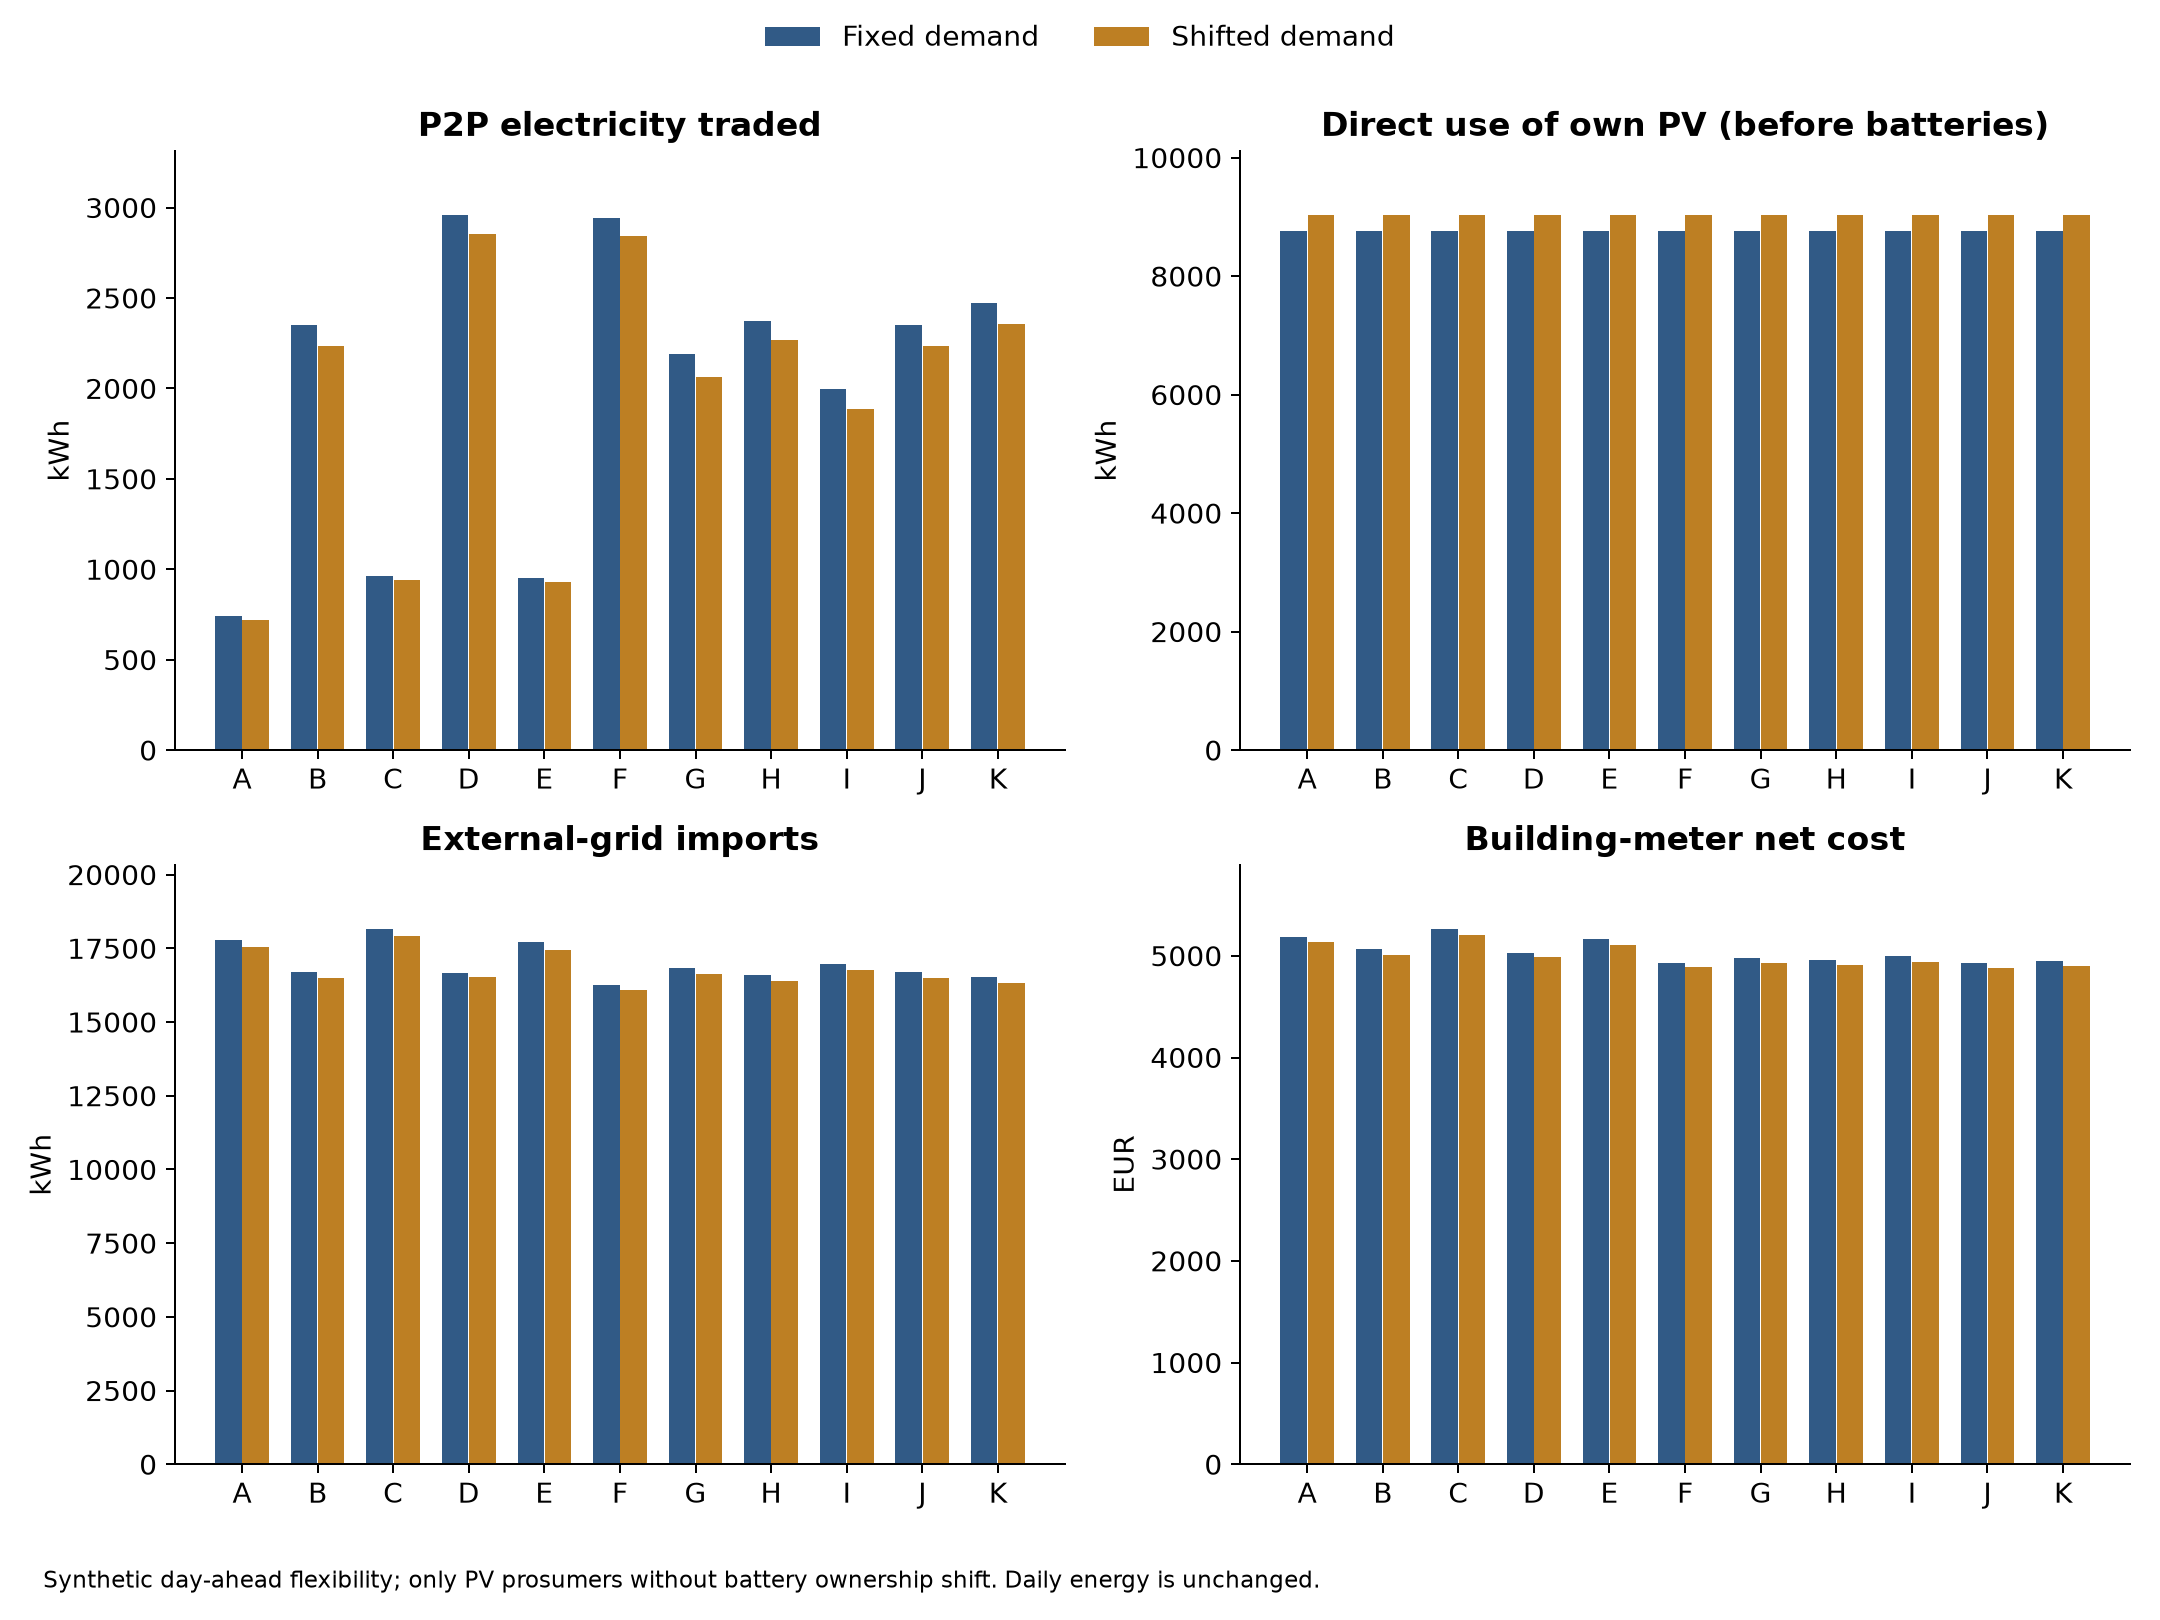
\includegraphics[width=\linewidth,height=0.45\textheight,keepaspectratio]{images/demand_response_comparison.png}\end{center}

{\small Figure 9. Paired scenarios hold PV, buildings, daily energy and market seeds fixed. Load timing changes only. Direct self-consumption excludes battery flows; meter cost includes fees/rewards. Synthetic simulation outputs.\par}
\par\medskip

Shifted energy: \textbf{353.804 kWh} across 43 meters. All daily demand is retained; unused flexibility stays at its original time.
\par\medskip

\begingroup\small
\begin{longtable}{>{\RaggedRight\arraybackslash}p{\dimexpr0.128205\linewidth-2\tabcolsep\relax}>{\RaggedRight\arraybackslash}p{\dimexpr0.285996\linewidth-2\tabcolsep\relax}>{\RaggedRight\arraybackslash}p{\dimexpr0.285996\linewidth-2\tabcolsep\relax}>{\RaggedRight\arraybackslash}p{\dimexpr0.299803\linewidth-2\tabcolsep\relax}}
\toprule
\textbf{Scenario} & \textbf{P2P fixed kWh} & \textbf{P2P shifted kWh} & \textbf{Change kWh} \\ \midrule
\endfirsthead
\toprule
\textbf{Scenario} & \textbf{P2P fixed kWh} & \textbf{P2P shifted kWh} & \textbf{Change kWh} \\ \midrule
\endhead
A & 863.982 & 847.031 & -16.951 \\ \addlinespace[3pt]
B & 2,858.451 & 2,699.393 & -159.058 \\ \addlinespace[3pt]
C & 1,047.066 & 1,004.087 & -42.979 \\ \addlinespace[3pt]
D & 3,523.217 & 3,357.257 & -165.960 \\ \addlinespace[3pt]
E & 1,030.768 & 993.673 & -37.095 \\ \addlinespace[3pt]
F & 3,473.971 & 3,306.066 & -167.905 \\ \addlinespace[3pt]
\bottomrule
\end{longtable}
\endgroup

{\small P2P volume falls in 6 of 6 recorded pairs. Direct own-PV use rises by the shifted energy. Better self-consumption and maximum P2P are different objectives. Run: python main.py --include-priority --compare-demand-response\par}
\par\medskip

\clearpage

\section*{24  Team guide: what changes in daily behavior}
\par\medskip

Fixed demand follows building use, regardless of sunshine. With demand response, an eligible prosumer plans a limited part of its electricity use around its own PV forecast. Examples might include flexible laundry or controllable cooling, but these are interpretations: the code moves divisible energy rather than scheduling identified appliances.
\par\medskip

\begin{center}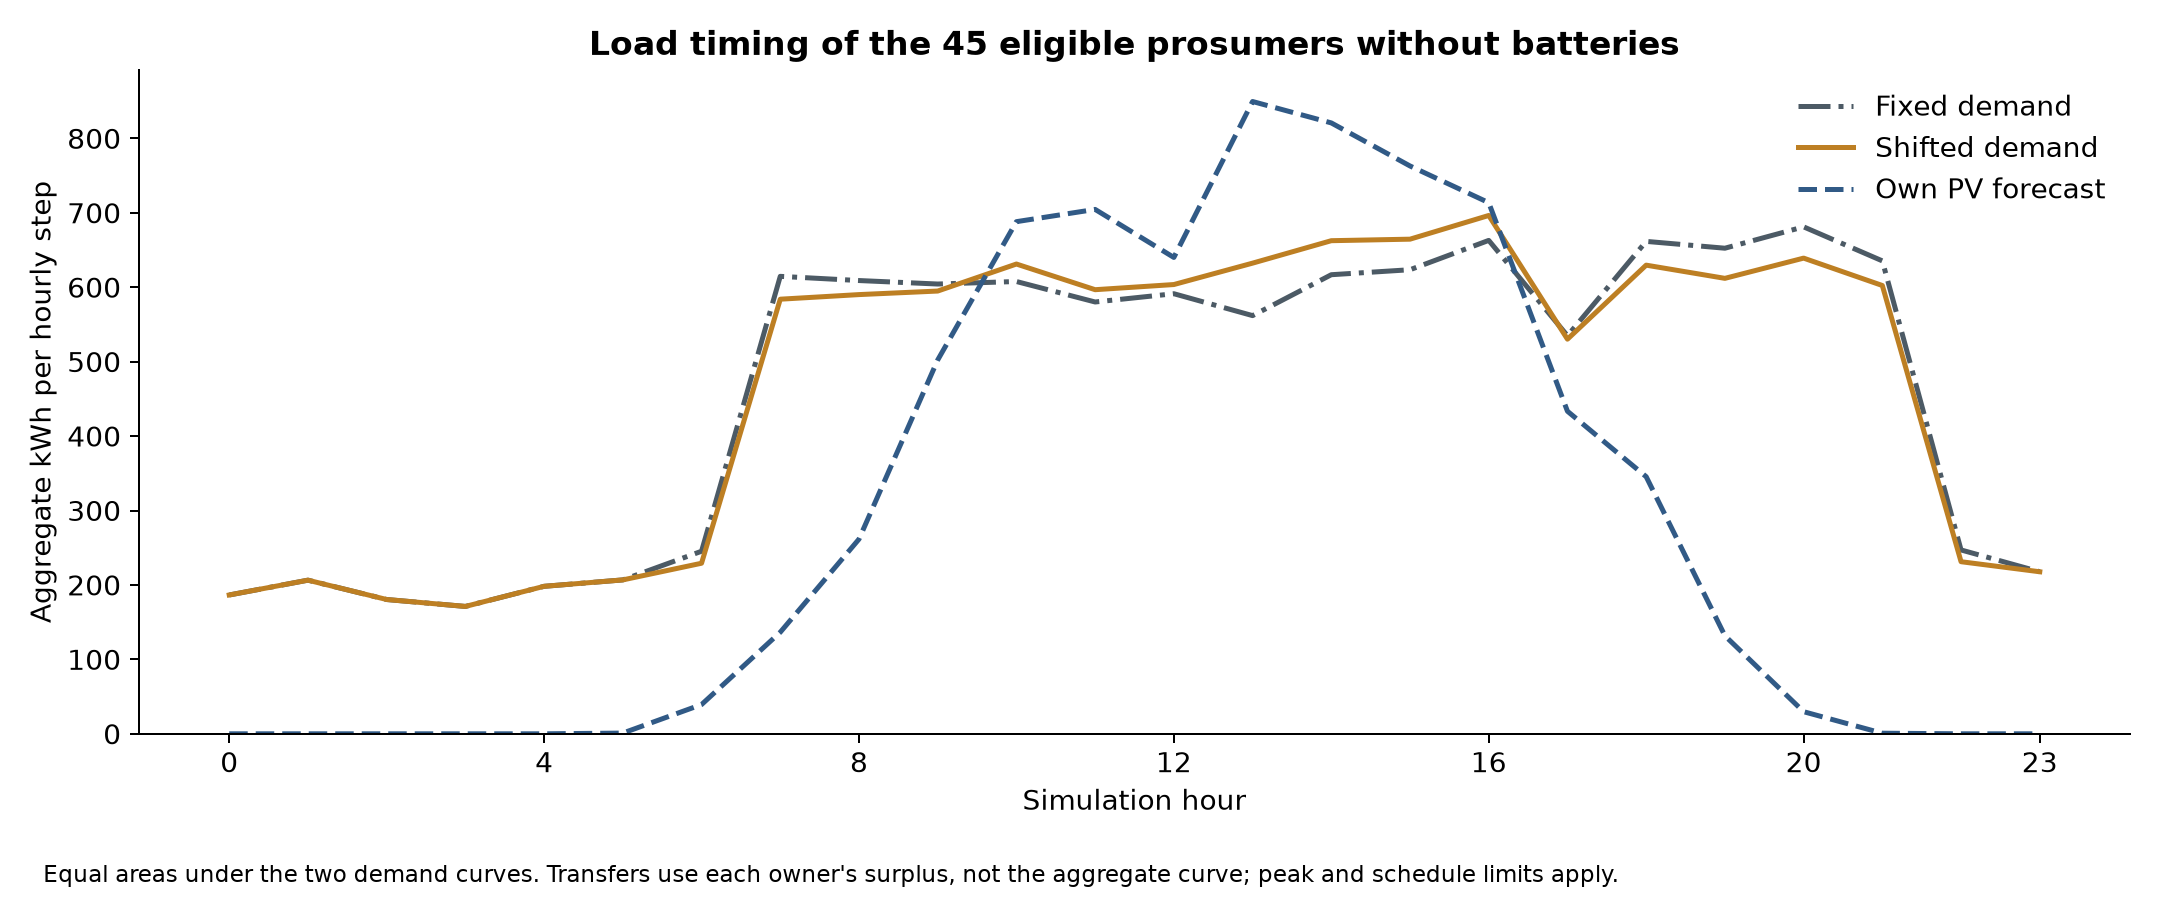
\includegraphics[width=\linewidth,height=0.45\textheight,keepaspectratio]{images/demand_response_hourly.png}\end{center}

{\small Figure 10. Aggregated forecasts for the 45 eligible prosumers. Both demand curves have the same daily area. The blue curve is unchanged PV. Matching is performed separately for each owner, so surplus in one building cannot justify shifting load in another.\par}
\par\medskip

\subsection*{How the day-ahead rule works}
\par\medskip

\textbf{1. Select eligible meters.} Only PV-equipped prosumers with no battery ownership participate. The 50 consumer-only meters and all 55 battery owners retain their demand. The same 45-meter eligibility applies to every A-F scenario; disabling storage in C/D does not silently add eligible meters.
\par\medskip

\textbf{2. Find flexible demand and own surplus.} For each complete local day, rank permitted source hours by forecast PV deficit. At a source hour, removable energy is the smaller of flexible\_fraction x original demand and original demand minus PV. This protects fixed demand and electricity already covered by PV.
\par\medskip

\textbf{3. Find a receiving hour.} Search hours no more than six hours earlier or later, on the same date and inside the allowed schedule. Prefer the largest remaining own-PV surplus. A receiving hour is limited by both unused PV and a maximum 50\% increase over its original demand.
\par\medskip

\textbf{4. Move what fits.} Record the source, target and quantity. Subtract and add exactly the same kWh. Any portion without a feasible destination stays at its original time. No cross-day transfers, electricity storage, grid charging or demand cancellation are introduced.
\par\medskip

\clearpage

\section*{25  Team guide: worked example and interpretation}
\par\medskip

\subsection*{Example: a house without a battery}
\par\medskip

\begingroup\small
\begin{longtable}{>{\RaggedRight\arraybackslash}p{\dimexpr0.266272\linewidth-2\tabcolsep\relax}>{\RaggedRight\arraybackslash}p{\dimexpr0.216963\linewidth-2\tabcolsep\relax}>{\RaggedRight\arraybackslash}p{\dimexpr0.516765\linewidth-2\tabcolsep\relax}}
\toprule
\textbf{Quantity} & \textbf{Illustrative value} & \textbf{Consequence} \\ \midrule
\endfirsthead
\toprule
\textbf{Quantity} & \textbf{Illustrative value} & \textbf{Consequence} \\ \midrule
\endhead
19:00 demand / PV & 10 / 0 kWh & At 20\% flexibility, at most 2 kWh can leave this hour. \\ \addlinespace[3pt]
13:00 demand / PV & 2 / 10 kWh & Own surplus is 8 kWh, but the 50\% rebound limit permits only 1 extra kWh. \\ \addlinespace[3pt]
Time distance & 6 hours & The target is permitted, provided both hours lie inside the configured window. \\ \addlinespace[3pt]
Actual transfer & 1 kWh & Demand becomes 9 kWh at 19:00 and 3 kWh at 13:00; daily energy is unchanged. \\ \addlinespace[3pt]
\bottomrule
\end{longtable}
\endgroup

The other 1 kWh of potential flexibility stays at 19:00 if no other destination is feasible. Direct own-PV use rises by 1 kWh; available PV surplus falls by 1 kWh. This example explains the algorithm and is not a measurement from a particular simulated building.
\par\medskip

\subsection*{Building-type assumptions}
\par\medskip

\begingroup\small
\begin{longtable}{>{\RaggedRight\arraybackslash}p{\dimexpr0.236686\linewidth-2\tabcolsep\relax}>{\RaggedRight\arraybackslash}p{\dimexpr0.177515\linewidth-2\tabcolsep\relax}>{\RaggedRight\arraybackslash}p{\dimexpr0.216963\linewidth-2\tabcolsep\relax}>{\RaggedRight\arraybackslash}p{\dimexpr0.368836\linewidth-2\tabcolsep\relax}}
\toprule
\textbf{Type} & \textbf{Flexible fraction} & \textbf{Allowed hours} & \textbf{Meaning} \\ \midrule
\endfirsthead
\toprule
\textbf{Type} & \textbf{Flexible fraction} & \textbf{Allowed hours} & \textbf{Meaning} \\ \midrule
\endhead
Small house & 20\% & 06:00-23:00 & Most load stays fixed; a bounded share can move. \\ \addlinespace[3pt]
Apartment block & 15\% & 06:00-23:00 & Aggregate flexibility across flats; no individual appliance model. \\ \addlinespace[3pt]
Supermarket & 5\% & 07:00-22:00 & Most load remains fixed; refrigeration is not freely rescheduled. \\ \addlinespace[3pt]
School & 10\% & 08:00-17:00 & Only permitted operating periods; closed weekends do not shift. \\ \addlinespace[3pt]
\bottomrule
\end{longtable}
\endgroup

All percentages are proposed engineering defaults. Actual building-type opening/closing times further constrain nonresidential windows. They require calibration before making claims about real users; comfort, thermal dynamics, task deadlines, occupant consent and device-level minimum run times are not modeled.
\par\medskip

\subsection*{How to interpret and audit the result}
\par\medskip

Higher direct self-consumption can leave less PV for neighbors, reducing P2P kWh even when household imports fall. Always compare absolute P2P volume, its changing surplus denominator, direct own-PV use, grid flows and both cost boundaries. Do not compare a shifted regulated run with an unshifted unregulated run and attribute both changes to regulation.
\par\medskip

Fixed outputs remain in results/; shifted outputs are in results/demand\_response/. The paired CSV/JSON is demand\_response\_comparison. Inspect inputs/demand\_shifts.csv and hourly\_inputs\_baseline.csv in the shifted folder to trace each transfer. The model uses supplied forecasts, not future actual measurements; incomplete calendar days remain unchanged.
\par\medskip
\end{document}
